%******************************************************************
%******************************************************************
\chapter {Applications in X-ray Imaging}
%******************************************************************
%******************************************************************
\label{applications}


In this chapter we show the application of the developed \opticalflow and data analysis methods on a number of scientific problems from different research fields. For each application we start by giving a short introduction to the subject of investigation. We describe important aspects of the X-ray imaging setup and sample preparation. Then, we give a short description of a problem and specify our tasks for data processing. We evaluate each dataset according to our data taxonomy presented in Section \ref{data_taxonomy}. Then we provide a detailed discussion on the usage of appropriate data preprocessing  routines, derive a suitable \opticalflow model, optimize model parameters and perform data analysis, visualization and interpretation of the results.



%--------------------------------------------------------
\section{Motion Analysis}
%--------------------------------------------------------

\subsection{Particles Fluid Dynamics in Semi-Solid Metals}

\subsubsection{Introduction}

Semi-solid metals are two-phase mixtures, which exhibit unusual rheological properties \cite{Flemings91}.
Without stress they behave like elastic solids, but when a shear force is applied a transition into a viscous mixture takes place. 

The transition from a solid phase filled by liquid to a viscous state is accompanied by the breakup of
the solid skeleton into individual particles and clusters which can flow independently. This breakup process is known as a \textit{thixotropic effect} \cite{Spencer72}. In comparison to high pressure die casting, semi-solid casting (SSC) is performed at lower temperature conditions, which has a number of advantages \cite{Zabler13}. 

The liquid phase is well-studied and can be described as a Newtonian fluid. However, the flow properties and rheology of a solid-liquid mixture are poorly understood. As an example, such characteristics as size and distribution of particles and their clusters, flow properties, morphology of particle groups and events of breaking apart and solidify are crucial to be considered for semi-solid casting.  

A typical approach to study rheology of semi-solid metals is to use experimental rheometers by measuring viscosity of a system. With the use of this technique systematic studies were performed to evaluate the dependence on various parameters.  However, these studies are only statistical and do not provide enough information to describe and predict the actual casting process. 
Therefore, in order to investigate more complex phenomena an \textit{in situ} imaging method is required. For this purpose  X-ray imaging
methods are highly appropriate due to the penetrating
ability of the radiation.






\subsubsection{Experimental Setup}

The experiment was performed at a beamline station ID15a of the European Synchrotron Radiation Facility (ESRF). For our experiment a high absorption contrast is required to allow for high acquisition rates. For this purpose the high flux beamline ID15a was chosen to carry out this study.
ID15a beamline was operated in a white beam mode: the radiation from the source was filtered by approximately 20 mm of silicon, resulting in a photon flux density of approximately $10^{15}$ photons/mm/s.

The X-ray detector was an indirect system: an optical lens projects the luminescence image of a scintillator screen via a mirror system onto the sensor of a CMOS camera.  In order to acquire images with high frame rates, a Photron SA1 camera is used, which is based on a CMOS
sensor with 1024 $\times$ 1024 pixels (size 20 $\mu$m) and a true dynamic range of 800:1 grey levels (10 bit, with a 12 bit digitalization) (see Section \ref{digital_image} for details).

The experimental setup is shown in Figure \ref{fig:app_thixo_setup}.
It consists of an \textit{in situ} furnace with a linear motor driving injection of the sample material and an imaging system. The furnace is an
aluminium case covered with vermiculite plates to shield the heat 
produced by four Osram Xenophot 64635 HLX heating lamps (150 Watts, 15 Volts). A sheet of stainless steel is attached to a linear stepping motor and serves as a piston, pushing downwards into the sandwich structure at 20 mm/s velocity,
thereby injecting the semi-solid material into the channel.

\begin{figure*}[ht]
  \centerline{
    \mbox{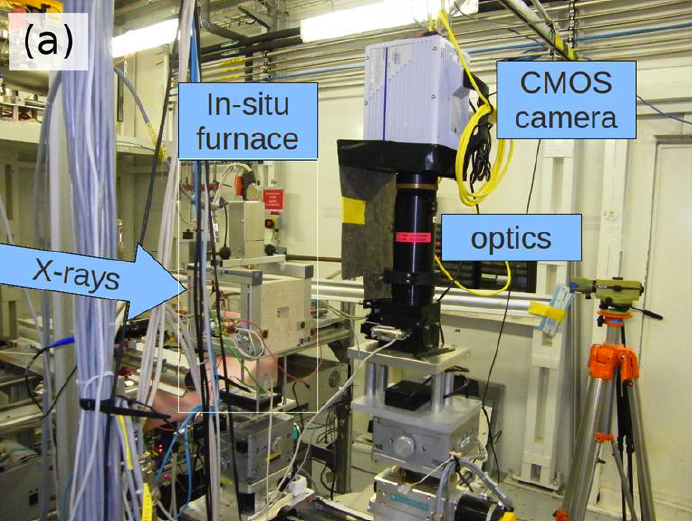
\includegraphics[scale = 0.314]{figures/app_thixo_setup1.PNG}}
    \mbox{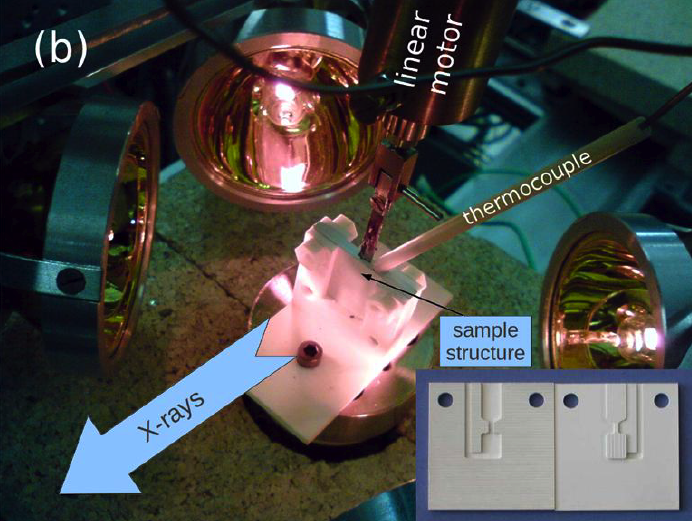
\includegraphics[scale = 0.314]{figures/app_thixo_setup2.PNG}}  
  }  
  \caption{Setup for fast radiography experiment on semi-solid alloys. \textbf{(a)}  Experimental hutch of the ID15a high energy beamline at the ESRF synchrotron facility with an in-situ furnace and a detector system. \textbf{(b)}
Close-up view into the sample environment: open in-situ furnace, four Xenophot heating lamps, a linear stepping motor drives down the piston into the
sandwich structure, thus injecting the semi-solid material during in-situ experiment. Image: \cite{Zabler13}}.
  \label{fig:app_thixo_setup}
\end{figure*}

The alloy Al-Ge32(wt.) was chosen for the experiment. The temperature for the SSC process is 420C for solidus temperature and liquidus temperature of 550C. After each experiment the samples were cooled down at the room temperature, extracted from the sandwich structure and carried for metallographic investigation under the light microscope (see Figure \ref{fig:app_thixo_radios}). Further details on sample preparation and sample environment can be found in the original publication \cite{Zabler13}.

\begin{figure*}[ht]
  \centerline{
    \mbox{\includegraphicslabeledw[scale = 0.30]{figures/app_thixo_radios1.PNG}{a}}
    \mbox{\includegraphicslabeledw[scale = 0.30]{figures/app_thixo_radios2.PNG}{b}}  
  } 
  \vspace{3pt}
  \centerline{
  	\mbox{\includegraphicslabeledw[scale = 0.30]{figures/app_thixo_radios3.PNG}{c}}
  	\mbox{\includegraphicslabeledw[scale = 0.30]{figures/app_thixo_radios4.PNG}{d}}  
  }  
  \caption{Radiographic sequence showing frames 250, 350 and 450 of the right-angle turn geometry. Images from \textbf{(a)} to \textbf{(c)} are 0.2 seconds apart. \textbf{(d)} Metallographic section obtained after the experiment to verify structural changes. Image: \cite{Zabler13}.
  \label{fig:app_thixo_radios}}
\end{figure*}


The employed Photron SA1 camera can acquire up to 5400 images/s in a full frame
mode. Due to the optical magnification, the detector system operates with an effective pixel sampling of 5.5 $\mu$m, which results in a spatial resolution of R $>$ 11 $\mu$m (see Section \ref{digital_image}). For the current study the acquisition rate was 500 images/s for the bottle-neck geometry (Figure \ref{fig:app_thixo_radio_filtered}) and 1000 images/s for the right-angle (Figure \ref{fig:app_thixo_radios}). 



\subsubsection{Task for Data Processing}

The main task for data processing is a quantitative investigation of complex flow dynamics in semi-solid alloy systems. For this purpose we perform:
\begin{itemize}
	\item Quantitative motion estimation to measure  the velocity of solid particles, clusters and air bubbles.
	
	\item Visualize trajectories to reveal flow patterns and interesting events during the casting process.
	
	\item Perform motion-based segmentation (using magnitude of the flow or flow direction as a measure) to classify particles and allow for extensive morphological analysis.
	  
\end{itemize}

\subsubsection{Data Evaluation}


Prior to data processing and optical flow computation we perform an input data characterisation according to our data taxonomy \ref{data_taxonomy}:

\begin{itemize}
	\item \textit{Image noise}: The dataset contains high amount of noise due to non-optimal imaging conditions, in particular short exposure time. As a result we obtained image data which is contaminated with high amount of Poisson noise. Additionally, there is small amount of saturated ("dead") pixels within image data. A proper treatment of noise is mandatory. Moreover, an optical flow model which is robust under noise is required.
	
	\item \textit{Contrast level}:  The image contrast is low, the solid particles and air bubbles are hardly distinguishable from the background. A proper treatment of low-contrast data is needed.
	
	\item \textit{Object size}: The solid particles, clusters and air bubbles are of average size.  There are no small and large objects.
	
	\item \textit{Object distribution}: Particles are distributed normally. In some cases the objects are close to each other and in some cases they are distributed sparsely. The object distribution should not pose a concern for data processing. 
	
	\item \textit{Object details}: Individual particles are of a homogeneous contrast, no details are present. As a result, the main source of information for the data term are the boundaries of each particles. In the case of particle clusters, which are moving conjointly the amount of details is higher and is composed of details of each individual particle. In general, the amount of details within particles is not sufficient, that is why the appropriate design of the smoothness term becomes important.
	
	\item \textit{Image artifacts}: There are very strong variations of brightness both in the space and time. There artifacts may pose a major problem for the optical flow estimation. A proper data correction technique is mandatory.
	
	\item \textit{Motion type}: The motion model may be classified as rigid. However, most of the circular particles cannot undergo the rotational motion (it is not captured for circular shapes). More complex clusters of particles may rotate, which frequently occurs during the solidification stage.
	
	\item \textit{Motion range}: Motion of particles thorough out the process is slow, thanks to the correctly chooses parameters for data acquisition, which allowed adequately sample the process, yet avoid significant motion blur.
	
	\item \textit{Motion discontinuities}: There is a certain amount of discontinuities between the moving particles and clusters. However, this should not affect the computation of flow fields in a substantial way.  A more dangerous scenario is the presence of occlusions between moving particles and their clusters, which can happen on later stages of the thixocasting process.
\end{itemize}




A summary of evaluation of this dataset is given in Table \ref{tab:eval_thixo}.
\begin{table}[ht] \footnotesize
	\centering
	\caption{Evaluation of the semi-solid alloys dataset.}
	\begin{tabular}{ccc}
		\toprule
		\textbf{Image} & \textbf{Data}   & \textbf{Motion}   \\ 
		\midrule
		\cellcolor{bad} noise: high       & \cellcolor{good} size:  average  & \cellcolor{good}type: rigid    \\ 
		\cellcolor{bad} contrast: low      & \cellcolor{good} dist: norm            & \cellcolor{good} range: small  \\ 
		\cellcolor{bad} artifacts: brightness   & \cellcolor{bad}detail: low  &  \cellcolor{norm} disc: occlusions   \\ 
		\bottomrule
	\end{tabular}
	\label{tab:eval_thixo}%
\end{table}


\textbf{Requirements on the Results}
\\
\\
\textit{Accuracy}: For this dataset we do not need sub-pixel accuracy. The error in the range of 1-3 pixels is sufficient to accomplish the task for data processing.
\\
\\
\textit{Density}: Dense flow fields are not mandatory. The correct estimation of the flow vector for each particle is sufficient. The fact that this requirement is relaxed gives some degree of freedom for the data preprocessing step - we can use much stronger filters to get rid of noise and artifacts. 
\\
\\
\textit{Motion components}: The full flow is required, i.e. both the flow magnitude and the flow direction. 
\\
\\
\textit{Consistency}: We do not pose any consistency constraints.
\\
\\
\textit{Motion boundaries}: We do not aim to capture strict flow on the boundaries of particles and particle cluster. Again, this gives us the possibility to increase the influence of the smoothness term and outcome the problem of low feature details.
\\
\\
\textit{Computation time}: Computation time is not an issue, the processing is done offline.
\\
\\
\textit{Data size}: A typical size of a single image frame is 1024 $\times$ 1024 pixels. An image sequence can consist of up to 1000 time frames. There is no restriction on processing due to the size of the input data - both image pairs are fitted into the memory and the processing is done sequentially.    


 

\subsubsection{Data Analysis: Preprocessing}


In order to improve the raw data and meanwhile preserve spatial and temporal details we develop an preprocessing routine.
\\
\\
\textit{Flat- and dark-field correction}. The routine starts with dark field filtering (\ref{flat_field_correction}) to correct for the fixed-pattern noise, including "dead" and saturated pixels. Flat-field radiograms are not available for this type of experiment, which is a typical limitation for fast \textit{in situ} experiments. Thus, temporal brightness variations have to be corrected by a dedicated filtering step.
\\
\\
\textit{Artifacts removal}. Next we proceed with applying a 3D Hybrid median filter (Section \ref{noise_filters}) to eliminate the high contrast speckle noise and small image artifacts caused by dust and scratches on the scintillator screen. For this procedure a number of time-lapse frames are used (N = 5). The procedure effectively removes small artifacts.
\\
\\
\textit{Brightness variation correction}. In order to equalize  non-uniform brightness variations we perform an image leveling using the median filter with a large spatial mask (Section \ref{image_leveling}). This part of the filtering process removes varying large-scale brightness patterns, but retains local details. 
\\
\\
\textit{Noise removal}. Finally, we use an anisotropic diffusion filtering (Section \ref{noise_filters}) to eliminate the image noise and at the same time to enhance particle edges.
\\
\\
\textit{Background subtraction}. To improve visual appearance of the filtered radiographs we subtract background which contains no structural details to reveal only the semi-solid material. 

\noindent On Figure \ref{fig:app_thixo_radio_filtered}we show  the result of our preprocessing procedure.

\begin{figure*}[ht]
  \centerline{
    \mbox{\includegraphicslabeledw[scale=0.32]{figures/app_thixo_radio_orig.png}{a}}
    \mbox{\includegraphicslabeledw[scale=0.32]{figures/app_thixo_radio_filtered.png}{b}}
  }
  %\vspace{3pt}
  
  \caption{Preprocessing  of the original radiographic sequence. \textbf{(a)}  Original radiograph. \textbf{(b)} Filtered radiograph. The filtering procedure consists of noise removal, brightness normalization, anisotropic diffusion filtering and background subtraction.}
  \label{fig:app_thixo_radio_filtered}
\end{figure*}

\subsubsection{Data Analysis: Flow Computation}

In order to compute flow fields we employed an advanced optical flow model, which takes into account multiple image features (Section \ref{assumptions_on_multiple_image_features}) and a priori information about motion model. For the construction of the data term we assume the constancy of image brightness (Section \ref{brightness_constancy_assumption}) and constancy of spatial intensity
gradients (Section \ref{gradient}). This joined assumption is more suitable for the motion estimation, if there is a small amount of spatial images features and objects are of low contrast. To provide robustness against noise and data artifacts that remain after a preprocessing step, the data term is extended by a combined local-global approach (Section \ref{clg}). Since we do not aim to capture fine details of moving particles, air bubbles and particle clusters, and the correct estimation on a more coarse scale (particle shape) is sufficient, a large value of the integration parameter in the range of $\rho$=[0.7...1.5] can be used. 


For the motion constraint we choose a flow-driven smoothness approach (Section \ref{flow_driven}). The rather high image acquisition rate (500 images/s and 1000 images/s) results in a smooth gradual motion of the constituents, from
which we can benefit by introducing an additional spatio-temporal smoothness constraint (Section  \ref{spatial_temporal}). In this way, the final optical flow model takes into account motion between more than two successive frames (N = 3).
Furthermore, to separate the motion of the liquid front from the flow of adjacent particles, the
smoothness is adapted (see Section \ref{adaptive_smoothness}) to a spatial mask covering the air-liquid interface. 

In order to cope with a large range of flow velocities a coarse-to-fine computation strategy is used (Section \ref{multilevel}). In order to visualize the resulted flow fields we use a color pseudo coding, which indicates the direction by color and the velocity by its brightness.


\begin{figure*}[ht]
  \centerline{
    \mbox{\includegraphicslabeledw[scale=0.32]{figures/app_thixo_radio_filtered.png}{a}}
    \mbox{\includegraphicslabeledw[scale=0.32]{figures/app_thixo_flow.png}{b}}
    \mbox{\includegraphicslabeledw[scale=0.32]{figures/app_thixo_flow_trajectories.png}{c}}
  }
  %\vspace{3pt}  
  \caption{\todo{Put arrows as in paper, put scale} Flow computation during semi-solid casting using optical flow. \textbf{(a)} Filtered radiographic projection. \textbf{(b)}  Calculated flow map. According to the color wheel at the bottom right a color shows direction and brightness encodes velocity. Arrows: (1) air bubbles, (2) cluster of particles moving at high speed on the crest of the liquid front, (3) a static particle around solidified region, (4) slowly moving bulk skeleton. \textbf{(c)}  Projected average velocity, integrated from frame 50 to frame 250. It shows the curved trajectories of air bubbles, as well as several solid particle clusters which can be seen at the lower right.}
  \label{fig:app_thixo_flow}
\end{figure*}



\subsubsection{Data Analysis: Flow Analysis}

The results of optical flow computation on a bottle-neck sequence are shown in Figure \ref{fig:app_thixo_flow}. One can clearly distinguish between the liquid and the solid phase whereby the latter appears darker due to the lower
X-ray density of aluminium compared to the Ge-rich liquid matrix. Air bubbles are difficult to distinguish from aluminium particles. Compared to the latter, they descend at higher velocities and appear darker in the radiographs (arrow 1 in Figure \ref{fig:app_thixo_flow}b). \todo{Make arrows in figures} Two or three small clusters of solid particles detached from the bulk and move freely through the channel following the liquid-air interface (arrow 2 Figure \ref{fig:app_thixo_flow}b).
One isolated particle appears to be completely static on this frame (arrow 3). The expanding liquid forms a semi-circular crest of constant velocity, as it can be expected for a Newtonian fluid. The movement of the solid bulk in the upper part of the radiograph is slow, which is captured by the computed flow field in Figure \ref{fig:app_thixo_flow}c (indicated by arrow 4). Evaluating the quantitative flow amplitude the liquid is found to advance at a maximum speed of 3.1 mm/s, with the air bubbles descending at relatively high speed, up to 3.9 mm/s. The velocity of the particle cluster at the lower liquid-air interface is 1.6 mm/s, and the average speed of the solid bulk in the upper part of Figure \ref{fig:app_thixo_flow}b remains less then 0.3 mm/s. 

A projected time evolution of interior of semi-solid alloy is shown in Figure \ref{fig:app_thixo_flow}c. Here, the average velocity was projected for each pixel over several hundred time frames, i.e. integrating from frame 50 to frame 250, while removing the velocities of the liquid front with a automatically extracted contour mask. The resulting color-coded
velocity projection shows dynamics of solid particles, clusters and air bubbles. The latter follow a curved trajectory until the downwards directed pressure is balanced by the buoyant force and their motion describes a hook trajectory.


\begin{figure*}[ht]
  \centerline{
    \mbox{\includegraphicslabeledw[scale = 0.38]{figures/app_thixo_turbulence1.PNG}{a}}
    \mbox{\includegraphicslabeledw[scale = 0.38]{figures/app_thixo_turbulence2.PNG}{b}}
  }  
  \caption{Example of turbulent motion in the right angle turn channel. \textbf{(a)} Input radiograph with magnified region of
interest. \textbf{(b)} Color-coded turbulent motion of a single particle recorded over 23 frames. The arrows
indicate the direction of particle motion as well as the velocity amplitude (arrow length).}
  \label{fig:app_thixo_turbulence}
\end{figure*}

When the experiment is carried out with a different channel geometry (right-angle turn) the flow behavior changes dramatically. The right-angle mold geometry was chosen to create a more turbulent flow, in the hope that the flow of both liquid and solid phases would be more conjoint compared to the bottleneck geometry. 
Judging from the metallographic sections of the final structure (see Figure \ref{fig:app_thixo_radios}d) the solid phase appears indeed to stay closer to the liquid front. Furthermore, evaluation of visualized flow fields reveals numerous particles which exhibit turbulent, Brownian-like motion. An example of such event can be seen in Figure \ref{fig:app_thixo_turbulence}. 


A spontaneous break-up of a larger particle cluster from the solid skeleton is displayed in Figure \ref{fig:app_thixo_break}. A large region of the solid phase, approximately 1.5 mm in diameter remains frozen for approximately
35 ms (Figure \ref{fig:app_thixo_break}), then suddenly the upper half of this cluster moves at high speed into separate directions, indicated by velocity magnitude flares, while the lower part of material remains still.



\begin{figure*}[ht]
  \centerline{
    \mbox{\includegraphicslabeledb[scale=0.22]{figures/app_thixo_break1.png}{a}}
    \mbox{\includegraphicslabeledb[scale=0.22]{figures/app_thixo_break2.png}{b}}
    \mbox{\includegraphicslabeledb[scale=0.22]{figures/app_thixo_break3.png}{c}}
  }
  %\vspace{3pt}  
  \caption{Example of sudden breakup of a larger cluster of particles, visualizing thixotropic effect. Images show radiographs of the right-angle turn geometry with the super-imposed velocity amplitude with brightness. \textbf{(a)} Frame 270, rectangle indicates a region where only little motion of the solid phase is observed. \textbf{(b)} In frame 296 the solid skeleton in the same region has become complete static (i.e. solidifies). \textbf{(c)} 34 frames later (frame 330, 35 ms apart) the static structure breaks up into many parts.}
  \label{fig:app_thixo_break}
\end{figure*}


%\comment{\subsubsection{Data Analysis: Motion-based Segmentation}}
%
%\comment{Make it. Motion-based Segmentation including Particle Analysis.}
%
%


\subsubsection{Results}

\textit{In situ} experiments by means of fast X-ray radiography with the optical flow analysis revealed a multitude of dynamical effects, particularly for right-angle turn geometry of the flow channel. Here, isolated turbulent particle motion and transition from a frozen solid skeleton to moving particle / clusters could be observed. This, we believe, is the \textit{first visual proof} of the thixotropic break-up during semi-solid injection. 

For the bottleneck channel in the narrow part only few particles traverse the bottleneck, the remains accumulate at the entrance. The solid movement comes to a complete halt, when the liquid has fully filled the recipient and compressed solid particles block further flow through the channel. Our results clearly show the inter-particle as well as the particle-wall friction to be the hindering force during semi-solid injections through thin cavities.

On the contrary, both solid and liquid phase moved relatively conjointly through the right-angle turn in the second experiment, which was found to locally exhibit turbulent flow resulting in Brownian-like particle motion and breakup of larger clusters into smaller particles. It appears that the less laminar flow of the liquid which takes place in such channel-turns and -corners allows the solid skeleton to advance at a similar speed with the liquid. 

These investigation extended by others geometries or introduction of additional compounds, as well as temperature dependence studies should advance the understanding of semi-solid casting technology.  









%--------------------------------------------------------
\subsection{Analysis of Morphogenesis in Frog Embryos}
%--------------------------------------------------------

\subsubsection{Introduction}

A primary goal in biology is to understand the behavior of cells during the development of an organism. One way to reach it is to image the actual morphological changes of embryonic structures \textit{in vivo} with sub-cellular resolution. Many morphogenetic events take place in the process of embryogenesis. One particularly important stage is \textit{gastrulation}, a stage when a series of dramatic changes occur and coordinated cell movements results in a transformation of a simple, homogeneous ball of cells into a complex multi-layered organism \cite{Keller03}. 

In model organisms, such as \textit{Xenopus laevis} and zebrafish, cell movements, tissue and organ formation have been studied by a number of well-established imaging methods: microscopy for explants and fixed embryos, \textit{in vivo} using fluorescence microscopy \cite{Keller08, Huisken09} or microscopic magnetic resonance imaging \cite{Papan07}. However, these methods do not allow to visualize \textit{in vivo} cell behavior in \textit{optically opaque} living embryos with micrometre-scale spatial resolution. 

To overcome these limitation we use in vivo time-lapse X-ray microtomography, based on a single-distance phase contrast and supplemented with a multi-scale motion analysis to examine the process of embryonic development. 

Phase-contrast imaging exploits high coherence and high intensity properties of the radiation produced by modern synchrotrons. During early developmental stages vertebrate embryos are composed of
light chemical elements (comparable with water). As a result, for hard X-rays phase changes in the transmitted wave dominate the effects of attenuation of the intensity. This allows to avoid high dose deposition attributed to a conventional X-ray absorption imaging, which is a crucial aspect for investigation of living organisms. Due to a high
penetration depth, high spatial and temporal resolution phase-contrast microtomography is a genuine 3D imaging modality to visualize the whole scale of embryonic structures: from organs, tissues and single cells, down to subcellular structures such as nuclei and yolk platelets.



\subsubsection{Experimental Setup}

The experiment described in this work was performed at beamline station 2-BM-B of Advanced Photon Source synchrotron facility (X-ray beam energy $E$ = 30 keV, photon flux density is $ \sim 10^{12}  \text{photons/s/mm}^2$). The experimental setup was optimized for a low dose deposition and longer observation time. Additionally, in order to avoid blurring artifacts due to cells motion and obtain sufficient image contrast a compromise between parameters of the acquisition process had to be made. After the phase retrieval algorithm was applied on projection radiography, a filter-back projection tomographic reconstruction method was used to obtain a 3D distribution of electronic density of the sample. The following parameters were used during the acquisition procedure: expose time per projection is 15 $ms$, number of projections $N=2000$, which yields a 18 $s$ acquisition time for one tomogram with the continuous rotation of the sample. To obtain a time-lapse images of the development process the waiting time between subsequent tomograms was 10 minutes. These time intervals were long enough to provide an adequate observation time and sufficiently short to result in a gradual cell movement between the subsequent time frames, which permits a reliable motion estimation. The steps of sample preparation, such as in vitro fertilisation, embryo culture and staging were carried out as described in \cite{Kashef09}. The X-ray phase-contrast microtomography setup is shown in Figure \ref{fig:app_embryo_setup}. 


\begin{figure*}[ht]
  \centerline{
    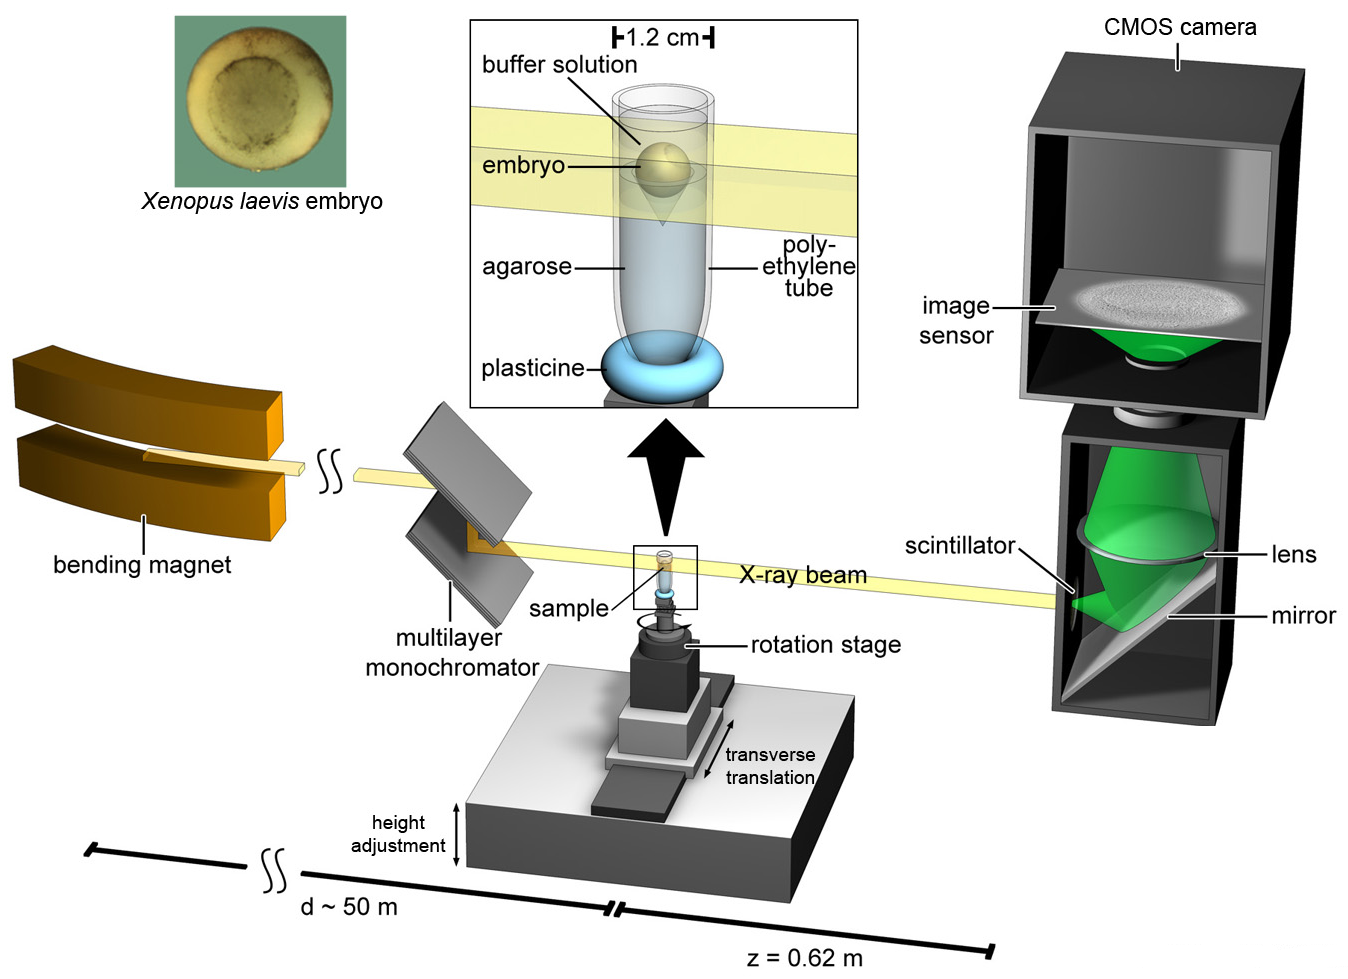
\includegraphics[scale = 0.25]{figures/app_embryo_setup.PNG} 
  }  
  \caption{Experimental setup for phase-contrast X-ray microtomography. A parallel photon beam is produced by a synchrotron source. A monochromator is used to change the properties of the beam. X-rays propagate over a distance $d=50 m$ and interact with a living Xenopus laevis embryo immersed in a buffer solution and suspended by agarose. The sample is mounted on a rotation stage to perform a tomographic scan. The 2D detector consists of a scintillator, converting X-rays into visible light, a mirror system, an optical lens, and a 
CMOS camera with 2016 $\times$ 2016 pixel resolution and pixel size 11 $\times$ 11 $\mu m^2$, \todo{Check correctness} which yields an effective pixel size of $\Delta x = 2.2 \mu m$.}
  \label{fig:app_embryo_setup}
\end{figure*}

Figure \ref{fig:app_embryo_renderings} shows 3D renderings of a mid-sagittally cut tomographic volumes of an embryo at the developmental stages 11.5, 12.0 and 12.5.
Single cells, tissue layers and important embryonic structures are distinguishable, including the
blastopore, archenteron, ventral and dorsal blastopore lips, blastocoel, blastocoel roof and floor, and the porous cell network between archenteron and blastocoel. A detailed, step by step protocol for the sample preparation, description of the experimental setup and data acquisition pipeline could be found in \cite{Moosmann14}. 

\begin{figure*}[ht]
  \centerline{
    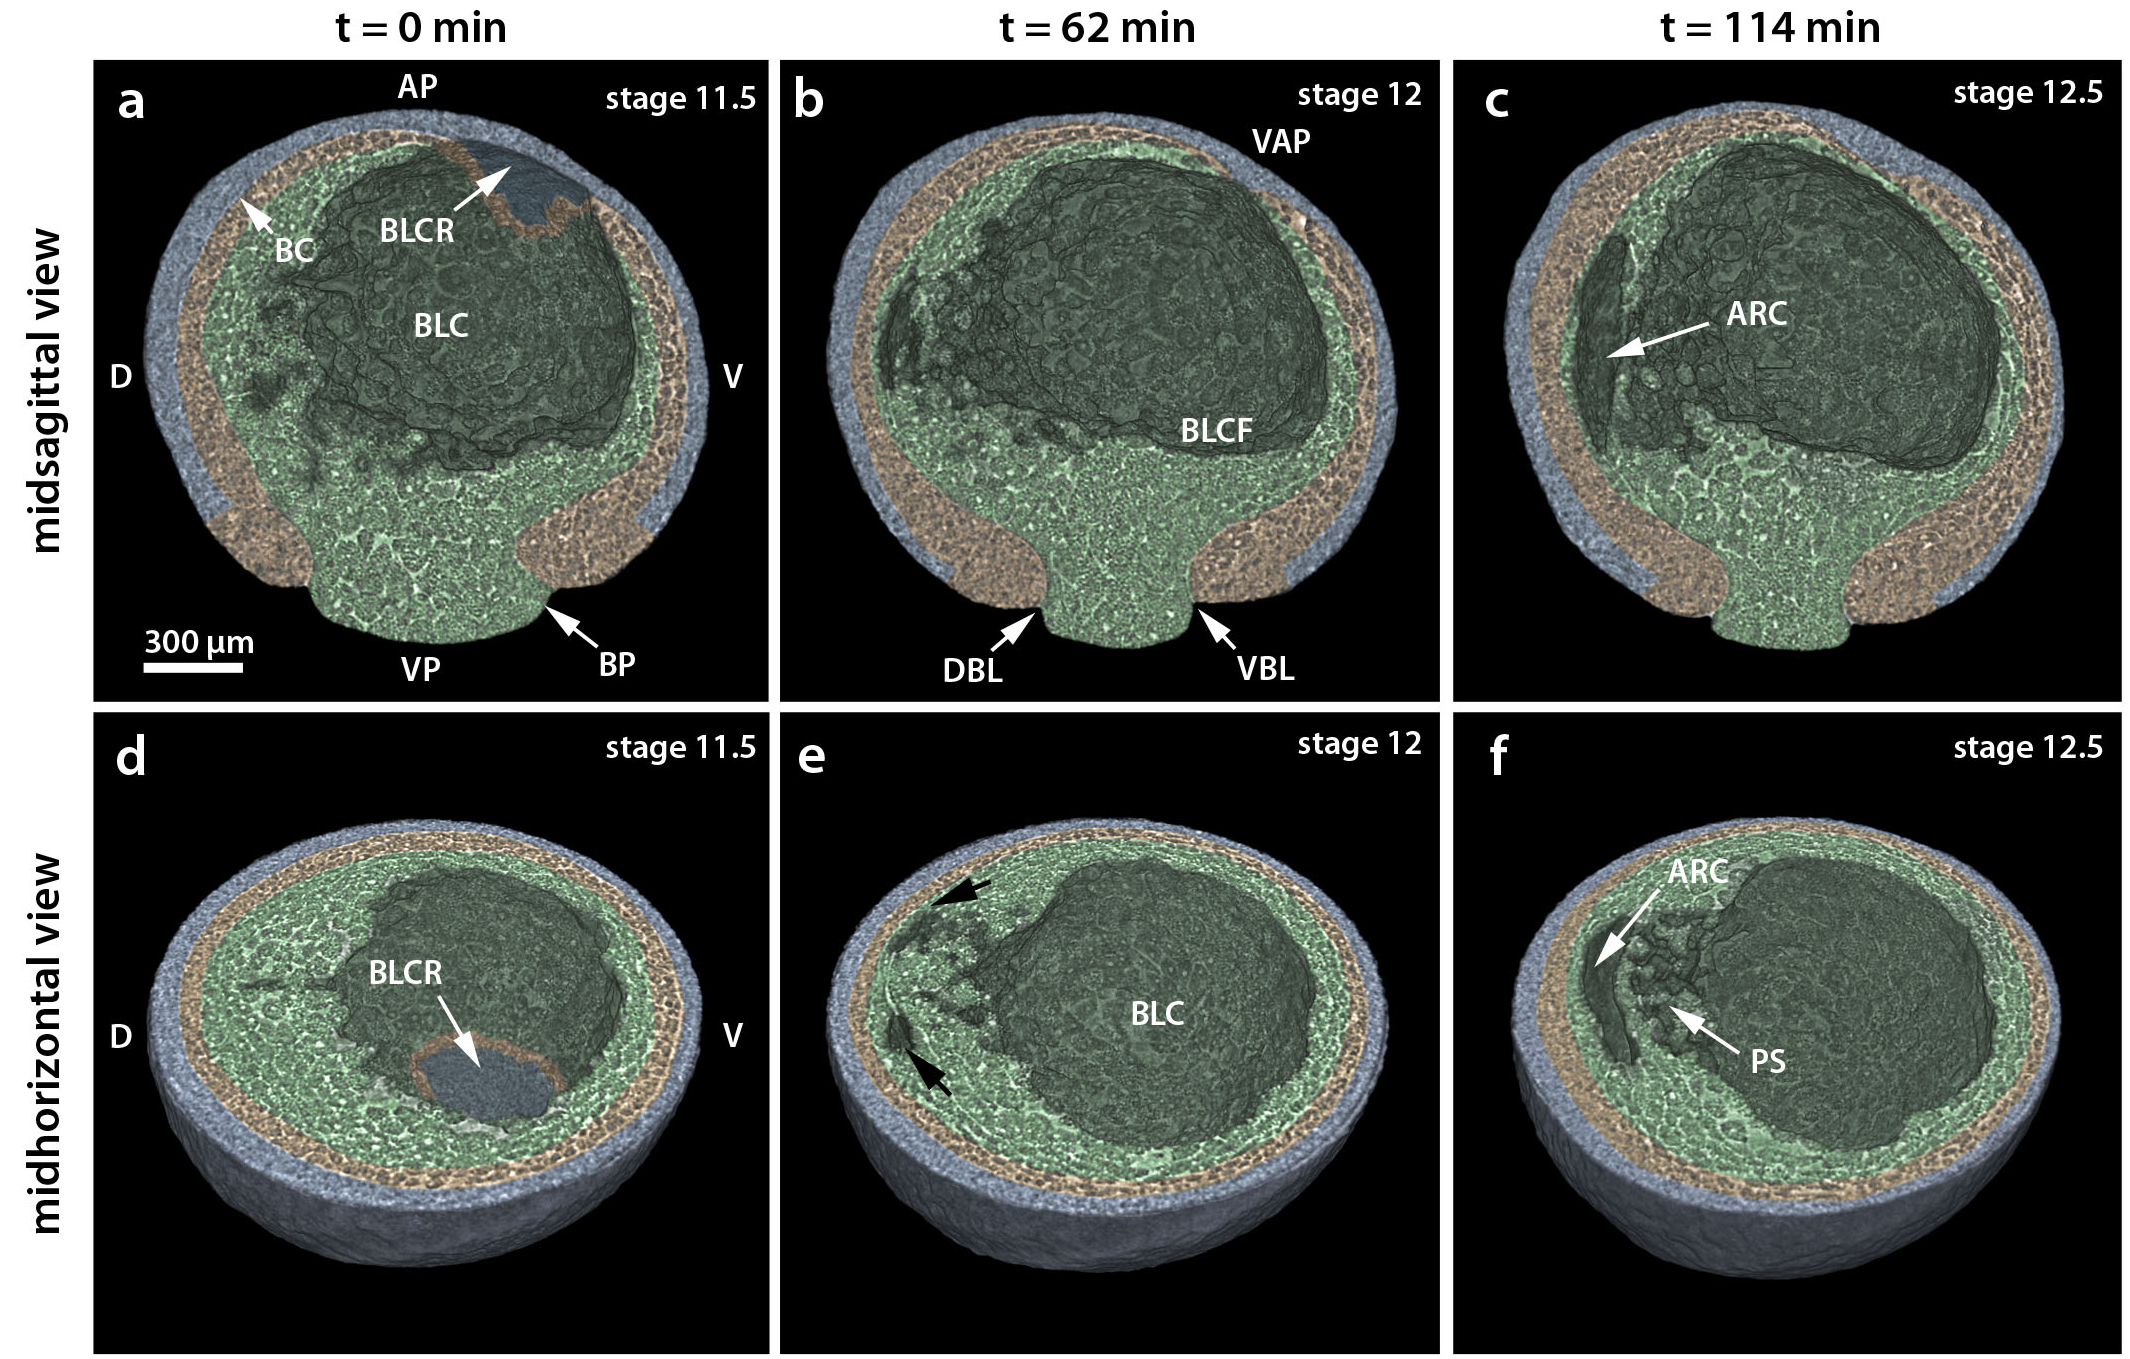
\includegraphics[scale = 0.22]{figures/app_embryo_renderings.PNG} 
  }  
  \caption{3D time-lapse series of \textit{Xenopus laevis} embryo during gastrulation stage. Mid-sagittal \textbf{(a-c)} and mid-horizontal \textbf{(d-f)} cuts of embryo 3D renderings
at stages 11.5 (0 min), 12 (62 min) and 12.5 (114 min). Tissue layers are labeled as follows:  ectoderm (blue),
mesoderm (orange), and endoderm (green). The following structures are identified:  Animal pole (AP), Archenteron (ARC),
Brachet’s cleft (BC), blastocoel (BLC), blastocoel floor (BLCF), blastocoel roof
(BLCR), blastopore (BP), dorsal and ventral sides (D, V), dorsal and ventral
blastopore lip (DBL, VBL), porous cell system between archenteron and
blastocoel (PS), ventral animal pole (VAP) and vegetal pole (VP).}
  \label{fig:app_embryo_renderings}
\end{figure*}



\subsubsection{Task for Data Processing}

Morphogenesis is a complex process, it involves many diverse and tightly coupled cell movements and tissue changes. The whole underlying dynamics can be captured by optical flow methods. To analyze the entire multitude of morphogenetic movements and events we use a multi-scale approach. In this approach we distinguish the following steps:
\begin{itemize}
	\item Perform dense, quantitative motion estimation of individual cells and tissues. Visualize global patterns of morphogenesis during mid-gastrulation stage.
	
	\item Distinguish collective motion and motion of individual cells. Discriminate between passive and active movements. Draw conclusions about cause-and-effect and dependency of morphogenetic processes.
	
	\item Track individual cells, analyze their dynamics to investigate interaction mechanisms between cells.
	
\end{itemize}


\subsubsection{Data Evaluation}

First, we evaluate our embryo datasets to identify possible problems and gather useful information for the design of an effective data processing pipeline. This data classification according to our data taxonomy \ref{data_taxonomy} reads:

\begin{itemize}
	\item \textit{Image noise}: The original radiograms contain high amount of noise due the short exposure time, which was necessary to limit radiation damage to the sample. After the tomographic reconstruction the noise issue is partially solved. However, the data may still suffer from the presence of noise, that is why optical flow models which are robust with respect to noise should be used. 
	
	\item \textit{Contrast level}:  The image contrast in the reconstructed tomograms after the phase-retrieval is sufficient.  It is possible to distinguish between tissues, organs, individual cells and even subcellular structures, such as nuclei. The good constrast level is strong point of the dataset. (See Figure \ref{fig:app_embryo_flow_analysis} a).
	
	\item \textit{Object size}: The structures of each tissue or organ are individual cells of different types. Most of the calls are small, some of the cells types (ectoderm) are even hardly resolved. The size of objects can be a major problem for optical flow estimation. (See Figure \ref{fig:app_embryo_flow_analysis} a).	
	
	\item \textit{Object distribution}: Cells are closely packed to form a tissue or an organ. The cells distribution can be classified as dense. Such allocation in a combination with the small size of cells pose a major challenge for data processing. (See Figure \ref{fig:app_embryo_flow_analysis}).
	
	\item \textit{Object details}: The amount of feature in tissues, organs or individual cells is high (except very small cells of ectoderm). Again, this property is a strong point of the dataset. (See Figure \ref{fig:app_embryo_flow_analysis} a).
	
	\item \textit{Image artifacts}: There are very strong variations of brightness in the original radiographs (See Figure \ref{fig:embryo_brightness_correction}). The variations appear as horizontal stripes which are shifting in time. The artifacts are severely degrading the original data. After the reconstruction brightness inhomogeneities cause very pronounced ring artifacts.  There artifacts pose a major problem for the optical flow estimation. The use of proper brightness and ring artifacts correction  techniques is mandatory.
	
	\item \textit{Motion type}: The motion of tissues, organs and individual cells is non-rigid. Cells may deform and change their shape. Such changes, however, do not occur rapidly and can be assumed to be locally smooth.
	
	\item \textit{Motion range}: Motion of cells is slow and there is not much variation in the motion range. The frame rate of the detector system was adequate to capture morphogenetic movements.
	
	\item \textit{Motion discontinuities}: There are a lot of motion discontinuities between the moving cells. Adjusted structures can move in completely different direction.
\end{itemize}




A summary of evaluation of embryo dataset is given in Table \ref{tab:eval_embryo}.
\begin{table}[ht] \footnotesize
	\centering
	\caption{Evaluation of the embryo dataset.}
	\begin{tabular}{ccc}
		\toprule
		\textbf{Image} & \textbf{Data}   & \textbf{Motion}   \\ 
		\midrule
		\cellcolor{norm} noise: average         & \cellcolor{bad} size:  small  & \cellcolor{norm}type: non-rigid    \\ 
		\cellcolor{good} contrast: high         & \cellcolor{bad} dist: dense            & \cellcolor{good} range: small  \\ 
		\cellcolor{bad} artifacts: brightness, rings   & \cellcolor{good} detail: high  &  \cellcolor{bad} disc: high   \\ 
		\bottomrule
	\end{tabular}
	\label{tab:eval_embryo}%
\end{table}


\textbf{Requirements on the Results}
\\
\\
\textit{Accuracy}: For this dataset we require accurate results. The error in the range of 1-2 pixels would be sufficient, but exceeding values should be eliminated from the results or indicated.
\\
\\
\textit{Density}: Dense flow fields are mandatory to capture differences in cells motion. 
\\
\\
\textit{Motion components}: The full flow is required, i.e. both the flow magnitude and the flow direction. 
\\
\\
\textit{Consistency}: We do not pose any consistency constraints.
\\
\\
\textit{Motion boundaries}: We aim to capture strict flow on the boundaries of moving cells. This information is crucial to analyze cell-to-cell behaviour.  
\\
\\
\textit{Computation time}: Computation time is not an issue, the processing is done offline. But taking into account he size of tomographic datasets (see next point), it would be a big advantage to perform the computation on GPU to speed up the process.
\\
\\
\textit{Data size}: The original size of a single tomogram is 2016 $\times$ 2016 $\times$ 2016, which corresponds to 32 Gb of floating-point data. This tremendous amount of data is impossible to process on CPU in a reasonable time. That is why data should be reduced or processed using GPU technology. Even in this case memory management is a major challenge.   



\subsubsection{Data Analysis: Preprocessing}
For the experiment described in this section the imaging conditions were optimized for a low-dose scenario and a strict compromise have been made between data quality and embryo viability. As a consequence, the dataset possess all kind of image degradation artifacts and is very challenging to analyze. 
Here we enlist data preprocessing steps to remove artifacts and improve signal-to-noise ratio as a preparation step for further data analysis. 
\\
\\
\textit{Removal of hot/dead pixels and brightness variations}. The procedure starts with a removal of hot and dead pixels (Section \ref{flat_field_correction}). A single dark field image $D$ is computed using a median of 60 dark-field images $D_1 ... D_{60}$, recorded independently (to acquire image statistics). \change{Then, flat-field images and original radiographs are dark-field corrected by taking a difference between the image $D$ every flat field image, as well as with the original radiograph.}
Due to cooling-induced thermal instabilities of the multilayer monochromator at the 2-BM-B beamline a temporally varying horizontal stripe brightness pattern significantly degrades the image quality. A crucial step is the correction of the initial radiographs and the flat-field images prior to any image reconstruction procedure.
\change{For this purpose before the flat-field correction grey values in each pixel along a given horizontal line are normalized to the mean value in this line} (Section \ref{image_leveling}). After the image leveling of flat-fields images a single flat-field image $F$ is calculated as a median. Normalized radiographs are then flat-field corrected using image $F$. Individual steps of the filtering procedure are shown in Figure \ref{fig:embryo_brightness_correction}.
\begin{figure*}[ht]
  \centerline{
    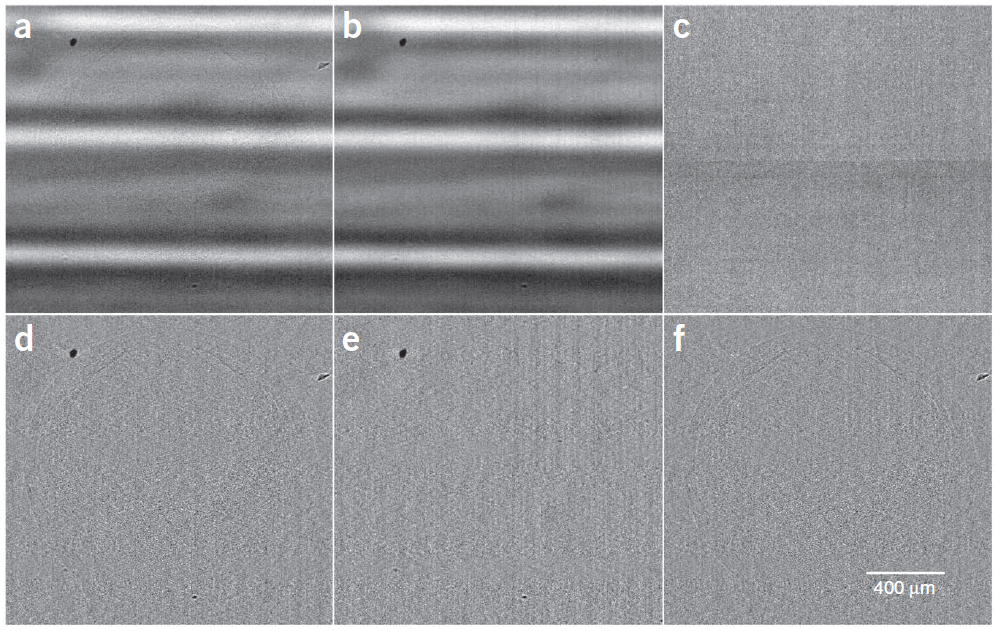
\includegraphics[scale = 0.55]{figures/embryo_brightness_correction.png} 
  }  
  \caption{Removal of brightness variation artifacts, flat-field and dark-field correction. \textbf{(a)} Raw projection radiograph. \textbf{(b)} Flat-field image. \textbf{(c)} Dark-field image.
\textbf{(d)} Projection radiograph with brightness artifacts removed. \textbf{(e)} Flat field image with brightness artifacts removed. \textbf{(f)} Flat- and dark-field corrected projection image with brightness artifacts removed.}
  \label{fig:embryo_brightness_correction}
\end{figure*}
\\
\\
\textit{Ring-artifact removal}. Because of short exposure times and, as a consequence, low count rates, the CMOS camera sensor produces characteristic vertical stripe artifacts. Since such patterns are sensor related and independent of the angle of rotation, they give rise to ring artifacts in the reconstructed volume. Ring artifacts can be effectively filtered in polar coordinates, in which circular brightness patterns become straight lines and can be easily identified. To implement this a filtering procedure is performed in the Fourier domain. As a first step, the Fourier transformation along horizontal and angular coordinates is done. Then, grey values of the plane corresponding to a zero angle are substituted by median values of adjacent planes \todo{reformulate, check refs}. As a final step, an inverse Fourier transformation is computed to obtain a stack of filtered sinograms. Figure \ref{fig:embryo_rings_removed} shows results of the ring artifacts removal procedure. 
\begin{figure*}[ht]
  \centerline{
    \mbox{\includegraphicslabeledw[scale = 0.45]{figures/embryo_rings_removed1.png}{a}}
    \mbox{\includegraphicslabeledw[scale = 0.45]{figures/embryo_rings_removed2.png}{b}}
    \mbox{\includegraphicslabeledw[scale = 0.45]{figures/embryo_rings_removed3.png}{c}}
  }  
  \caption{Removal of ring artifacts. \textbf{(a)} A horizontal slice through the reconstructed volume  (no ring artifacts filtering was used). \textbf{(b)} Reconstructed slice with the ring artifacts reduction procedure applied. \textbf{(c)} Difference between processed and unprocessed images shows the removed ring artifacts.}
  \label{fig:embryo_rings_removed}
\end{figure*}
\\
\\
\textit{Phase retrieval}. To extract a 3D distribution of refractive index a simple linear phase retrieval is performed \cite{Paganin98}.
\\
\\
\textit{Tomographic Reconstruction}. The final step of data processing is 3D  tomographic reconstruction using the filtered back-projection method (See Section \ref{computed_tomography}). Since the number of acquired projections is sufficient and an efficient data preprocessing pipeline is established, we achieve a good quality tomographic reconstruction. 


\subsubsection{Data Analysis: Flow Computation}

Even after an extensive pre-processing procedure, time-lapse sequences are still challenging to analyze in terms of automated techniques. For the reliable computation of flow fields we use a robust 3D variational optical flow method. For the modeling of the data term we choose the constancy of pixel brightness (Section \ref{brightness_constancy_assumption}). Since embryonic structures contain a lot of image details which are highly textured, and the grey value constancy assumption is more robust in the presence of noise, there is no benefit to use the gradient constancy assumption (as we concluded in our experimental evaluation). For the regularization of the motion field we use the flow-driven smoothness assumption (Section \ref{flow_driven}). 

Before motion computation the input images are smoothed using a Gaussian filter with a large spatial mask (optimal choice is in the range $\sigma=[1.2 \ldots 2.0]$).
To further improve the performance with respect to noisy data, we incorporate a local-global approach (Section \ref{clg}), that takes into account image data from a local neighborhood. The optimal values for the integration scale parameter are in the range $\rho = [0.5 \ldots 1.2]$. We use a multi-level
computation procedure (Section \ref{multilevel}) to capture the entire range of cell velocities. The number of warping levels and the warping scale parameter are the same as for the \textit{baseline} method (Section \ref{baseline_method}).  A median filtering of the flow fields at the intermediate computation levels is a crucial step to exclude data outliers due to the existing image artifacts. In general, we can also use a forward-backward checking as an automated confidence measure (Section  \ref{forward_backward_check}) to discard flow vectors which are not reliable. As a result of optical flow computation, we obtain a dense 3D velocity field, which we use for further analysis.  A visualization of the computed optical flow is given in Figure \ref{fig:app_embryo_velocity}, using sparse 3D vector glyphs. The assessment of the accuracy of the optical flow computation we present in the section, dedicated to cell tracking (See Section \ref{embryo_tracking}).

\begin{figure*}[ht]
  \centerline{
    \includegraphics[scale = 0.22]{figures/app_embryo_velocity.PNG} 
  }  
  \caption{3D time-lapse series of Xenopus laevis embryo during mid-gastrulation.
\textbf{(a-c)} Mid-sagittally  halved embryo renderings at stages 11.5 (0 min), 12 (62 min) and 12.5 (114 min). \textbf{(d-f)} Velocity fields on a 180-mm thick 3D slab centred about the cutting planes of \textbf{(a-c)}. Colour bar indicates velocity magnitude representation.}
  \label{fig:app_embryo_velocity}
\end{figure*}

\subsubsection{Data Analysis: Flow Analysis}

As  we already mentioned when stating the tasks for data processing , morphogenesis involves hierarchical, multi-scale cell movements. The whole range of underlying dynamics can be captured by the optical flow method and expressed as a dense motion field $\overrightarrow{v}$. We pursuit a multi-level strategy for motion analysis and investigate: i) global, collective aspects of the displacement field $\overrightarrow{v}$, ii) its local differential behavior and iii) a long range individual cells behavior using cell trajectories.

The computed motion fields for time-lapse series of \textit{Xenopus laevis} embryo during a mid-gastrulation  reveal global patterns of cell movements. These patterns comprise several morphogenetic processes, including rotation of the vegetal endoderm
(white arrowhead in Figure \ref{fig:app_embryo_velocity}g), involution of
the mesendoderm at the dorsal and ventral blastopore lips (white
arrows in Figure \ref{fig:app_embryo_velocity}d), and migration of the mesendoderm on the blastocoel roof towards the animal pole (red arrowhead in Figure  \ref{fig:app_embryo_velocity}d). By stage 12, prominent horizontal
movement within the endoderm layer is observed on the ventral side of the embryo (Figure \ref{fig:app_embryo_velocity}e). Additionally, a number of interesting events can be observed:  rapid migration of leading-edge head mesendodermal cells on the blastocoel roof, a bulk movement of the mesendoderm towards the animal pole, and local
cell dispersion due to the onset of archenteron formation. After the dorsal
and ventral edges of the mesendodermal mantle make contact and
cover the blastocoel, an overall halt of cell movements is observed on
the ventral side (Figure \ref{fig:app_embryo_velocity}f, stage 12.5). 
It is important to note, that before these studies, most of such morphogenetic processes in \textit{Xenopus laevis} were never captured \textit{in-vivo} and quantitatively analyzed with high resolution and accuracy.



For the next level in our hierarchical motion analysis approach, we examine a differentiated cell and tissue movements using a phase of the motion field (See Section \ref{phase}). This measure defined as a magnitude of the spatial gradient of the motion field $\textbf{v}=(v_x, v_y)$ and is given by $ P = |\nabla \textbf{v}|^2 $, where  $|f| = \sqrt{f^2_x + f^2_y}$ denotes the spatial magnitude and $\nabla = (\partial_{x}, \partial_{y})$ the spatial gradient.
Small values of measure $P$ indicate smooth, collective motion, while large values capture local changes in velocity magnitude and/or variations in the direction of $\textbf{v}$. In addition, we use a magnitude of the motion field $|\textbf{v}|$ (See Section \ref{magnitude}) to analysis an activity level of cells in a particular time point. 

\begin{figure*}[ht]
  \centerline{
    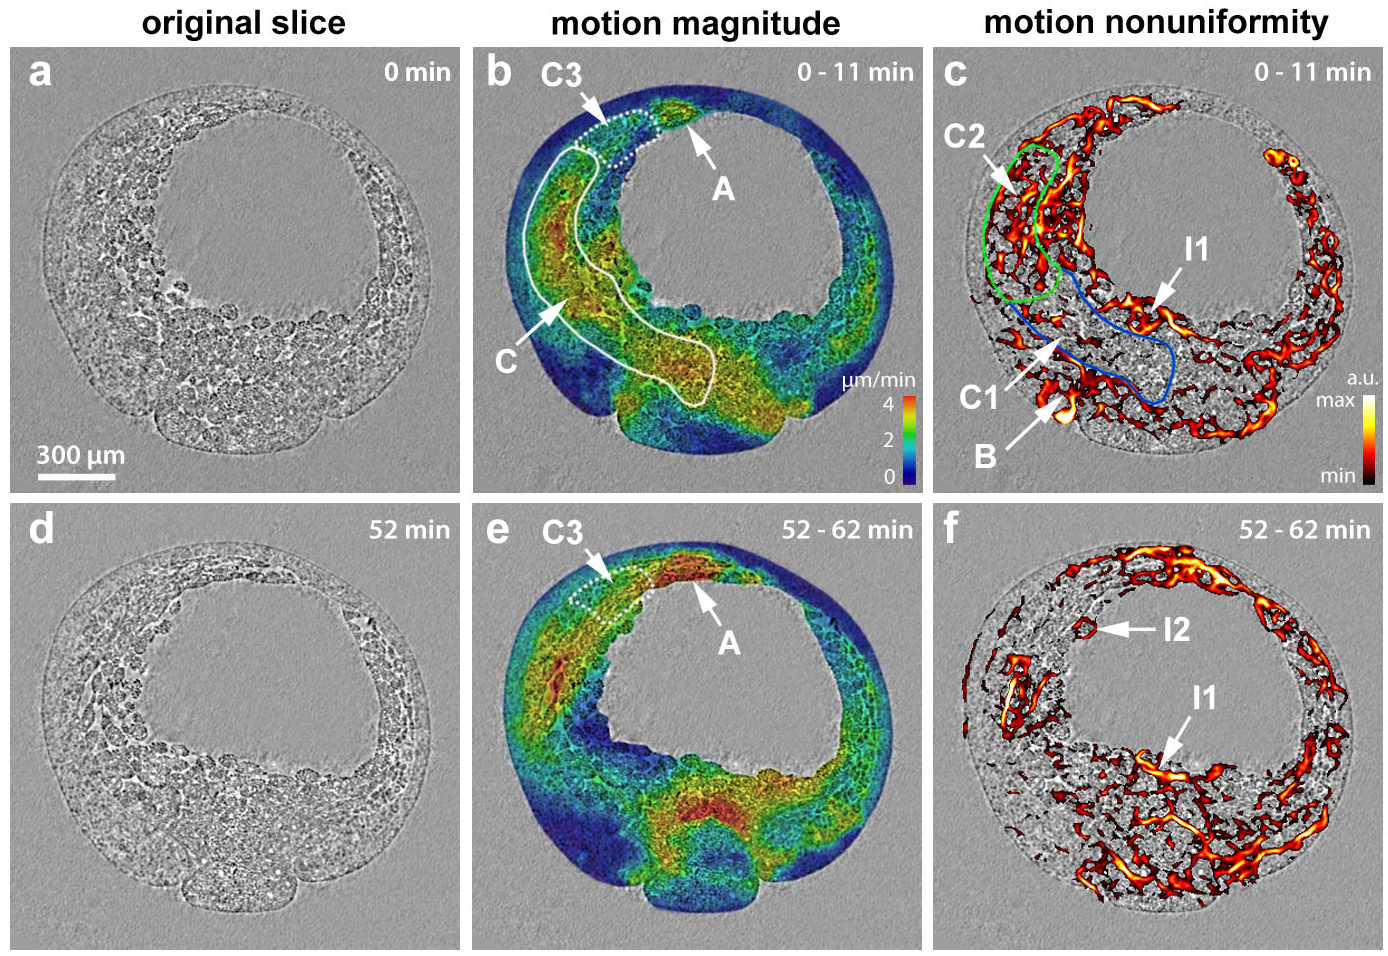
\includegraphics[scale = 0.333]{figures/app_embryo_flow_analysis.PNG} 
  }  
  \caption{Collective/differentiated motion and cells activity analysis. \textbf{(a, d)} 2D slices through tomographic volumes at times 0 and 52 min.  \textbf{(b, e)} Magnitude $|\textbf{v}|$ of the velocity field on a sagittal slice for two subsequent time frames. \textbf{(c, f)}: Field $P$ for the same slice and times frames.}
  \label{fig:app_embryo_flow_analysis}
\end{figure*}

Figure \ref{fig:app_embryo_flow_analysis} shows a mapping of magnitude and phase of the motion field measures. Using these visual maps it is possible to analyze, interpret and draw conclusions about casual relations between  different morphogenetic movements and events. Contour $C$ encloses a large, collectively moving cell mass
(Figure  \ref{fig:app_embryo_flow_analysis}a), extending from the vegetal region ($C1$, Figure \ref{fig:app_embryo_flow_analysis}c) along the
posterior–anterior axial mesendoderm and endoderm on the dorsal
side ($C2$, Figure \ref{fig:app_embryo_flow_analysis}c).



The movement of cells within the $C1$ region is mostly collective (small values of $P$), driven by blastopore closure. But in region the $C2$, a similar velocity magnitude is a result of involution of the dorsal mesendoderm (note the transition from $C1$ to $C2$ in Figure \ref{fig:app_embryo_flow_analysis}c).

Interestingly, despite the fact that the motion magnitude in region $C2$ is similar, cells do not move coherently. The relative cell motion within
$C2$ can be attributed to mediolateral intercalation associated with
convergent extension. This can explain the acceleration (Figure \ref{fig:app_embryo_flow_analysis} g, h) of
the anterior cells within $C$ (Figure \ref{fig:app_embryo_flow_analysis}a) towards the animal pole. Another interesting observation is a velocity gap (i.e. discontinuity) in region $C3$ (Figure \ref{fig:app_embryo_flow_analysis}a). It is seen from comparing Figures \ref{fig:app_embryo_flow_analysis}a and \ref{fig:app_embryo_flow_analysis}b in $C3$ region. This gap indicates active migration of the leading-edge cells in the
small region $A$ (Figure \ref{fig:app_embryo_flow_analysis}a,b) which was reported in the studies with explants.

Cells with individual movements are also discernible:  cells ($I1$) crawl on the blastocoel
floor (Figure \ref{fig:app_embryo_flow_analysis}c,d), and a single cell
($I2$) migrates on the endodermal cell mass (Figure \ref{fig:app_embryo_flow_analysis}f). 



\subsubsection{Data Analysis: Tracking}
\label{embryo_tracking}

In order to analyze individual cells behaviour for a longer time period we perform cell tracking. We use an automated tracking algorithm based on points tracking and optical flow (See Section \ref{tracking}).  Cell trajectories are obtained by time integration of a 3D flow field, starting with manually selected initial positions. As objects we identify the centers of  cell nucleus, lining both sides of archenteron walls (Figure \ref{fig:app_embryo_tracking}). We checked the accuracy of the optical flow algorithm by comparing automatically estimated cell trajectories with the corresponding trajectories tracked manually by the user expert. For an average traveled distance 58 $\mu$m over four successive volumes used for the trajectory computation, the average error was 4 $\mu$m, which roughly matches the resolution limit of 4.4 $\mu$m. This indicates a reliability of the optical flow computation.

\begin{figure*}[ht]
  \centerline{
    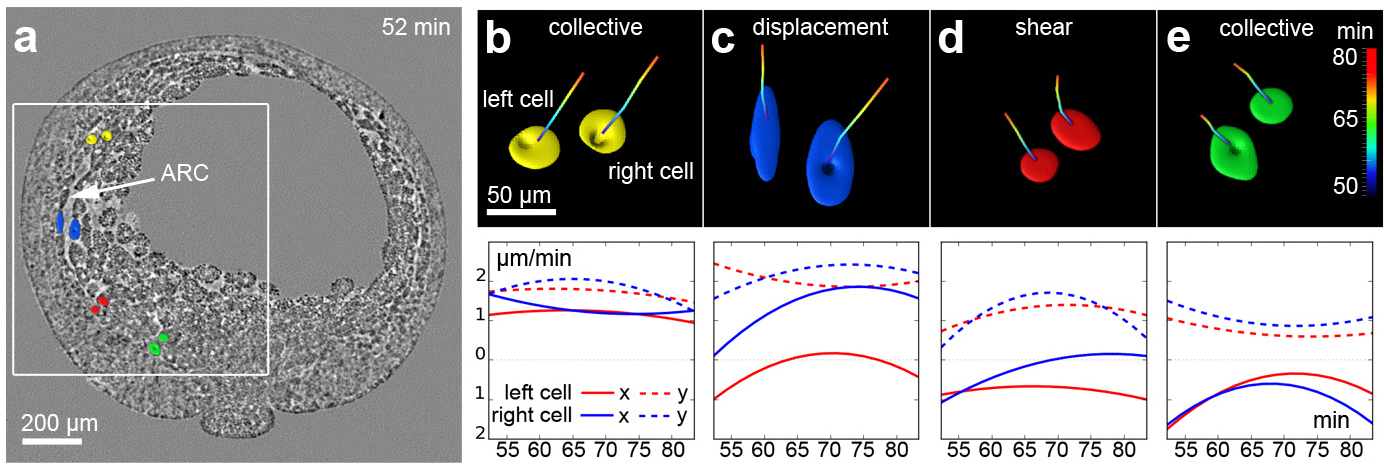
\includegraphics[scale = 0.33]{figures/app_embryo_tracking.PNG} 
  }  
  \caption{Trajectories and velocities of single cells lining the archenteron. \textbf{(a)} parasagittal slice at 52 min with highlighted cell pairs lining the region along the archenteron. \textbf{(b-e)}, trajectories of these cell pairs (top row) and associated velocity components in x-y (parasagittal) plane (bottom row; left cell: red, right cell: blue; solid: x-component, dashed: y-component).}
  \label{fig:app_embryo_tracking}
\end{figure*}

After trajectories of moving cells are estimated by our automated tracking procedure, parameters of their dynamics and interaction can be studied.
The two cell pairs most proximal to the animal pole (Figure \ref{fig:app_embryo_tracking}a,b) and the blastopore (Figure \ref{fig:app_embryo_tracking}a,e) display near-parallel trajectories in the direction of mesendodermal mantle, which is an indicator of collective motion.
In contrast, for cell pairs occupying more medial positions along the posterior-anterior extent of elongation a distinct directional variation is prominent (Figure \ref{fig:app_embryo_tracking}c,d).  For the anterior cells (Figure \ref{fig:app_embryo_tracking}c) there is a large difference between radial and tangential displacement. This large horizontal displacement is a consequence of the onset of archenteron inflation and vertical component is a result of active push from the side of vegetal cell mass. The dynamical characteristics are quantified and visualized in Figure \ref{fig:app_embryo_tracking}.


\subsubsection{Results}

The results presented in this section demonstrate that phase-contrast X-ray microtomography, combined with optical flow and multi-level motion analysis, is a powerful tool for 4D \textit{in vivo} investigation of embryonic
development. Analysis of differentiated motion allows to distinguish between active or passive tissue and cell movements, giving
insights into how collective morphogenetic events are powered by individual cell behaviour. Such studies can advance our understanding of the molecular mechanisms and biomechanical processes which drive embryogenesis.





%\subsection{Studying motion patterns of mating tsetse flies}
%
%\comment{Possibly could be skipped.}
%  
%\subsubsection{Introduction}
%
%An important and highly discussed question in morphological evolution of tsetse flies is why male genitalia diverge differently than other structures. 
%One of the suggestion is that male genitalia function are under sexual selection by female choice to induce female responses that will increase the possibility to fertilize the female's eggs.
%
%Testing this hypothesis has been difficult process because the inner structures are not visible and genital behavior of the coupling process in hidden inside the female.
%
%The current work aims to reveal completely new insights about functioning of male structures by the use of synchrotron X-ray imaging.
%
%\subsubsection{Scientific Task}
%Perform velocimetry analysis to study kinematics of motion patterns during coupling process.
%Study and highlight stereotyped, rhythmic movements of male's genitalia parts deep within the female organs. Distinguish the differences of the behavioral activity between different species. 
%
%\subsubsection{Scientific results}
%Optical flow computation is applied to a sequence of radiographic images to obtain dense displacement field between subsequent frames.
%In order to study kinematics of the particular genitalia parts the motion field could be visualized directly using vector representation.


%\subsection{Kinematics of feeding mechanisms in living insects}
%
%\subsubsection{Introduction}
%In insects, locomotory mechanisms such as walking or flying
%are well known for their highly coordinated nature; their rhythmicity
%and movement patterns are controlled by centralized neuronal circuits.
%This makes them ideal model systems for studying comparative functional morphology and biomechanics.
%
%\subsubsection{Scientific Task}
%Perform velocimetry analysis to study kinematics of feeding mechanisms in living insects.
%Highlight the mouthparts moving with the faster velocities on different feeding cycles.
%Analyze overall activity during the feeding process. Perform tracking of the individual mouthparts to analyze complex motion patterns. Use user-defined landmarks for the optical flow computation to adjust dense flow field computation with a ground truth tracking information provided by a user. 
%
%
%\subsubsection{Scientific results}
%Optical flow computation was applied to a sequence of radiographic images to obtain dense displacement field. In order to study kinematics of the particular mouthparts (acceleration, relative motion) magnitude of the motion field is superimposed with the original radiograph.
%
%In order to enhance the result of the optical flow computation we employ a semi-automated tracking approach, which is based on the combination of manual tracking information provided by the user and automatic optical flow computation. It is done by setting known landmarks directly to the computational scheme as a ground truth data. As a result, the optical flow computation is adopted and combined with a manual tracking information to provide much more reliable user-driven solution.



\section{Temporal Changes Detection}


\subsection{Stability Study During Foaming Process}
\label{application_foams}

\subsubsection{Introduction}

The production, characterization and application of foams and cellular structures has attracted increasing attention in the recent decade. Foams and cellular structures exhibit remarkable properties, such as high strength and mechanical stiffness, low density and the ability to absorb large amounts of energy. The porous materials are widely used for a broad range of industrial, medical and scientific applications.

During a foaming process a complex interplay of different physical phenomena takes place. Such processes include: liquid drainage,
coalescence, coarsening, topological reorganization, pore
inflation and many others. A sudden instability in a film leading to its disappearance is called \textit{coalescence}. Such process triggers two (or more) neighbor bubbles to merge onto a single one by the rupture of separating film walls. Coalescence events are the major phenomena which affects the spatio-temporal stability of the foam. 

An understanding of the underlying processes of foaming dynamics is a challenging task that is important for future technological progress.
Theoretical models of drainage and
coalescence are available in the literature \cite{Bhakta97, Ireland09}.  However, the adequacy of these models with real physical phenomena is still far from being completely established.
A number of experimental studies for different variety of foams have been performed to investigate coalescence events, for example, using
conductivity profiles, acoustic measurements, neutron and visible-light scattering \cite{Myagotin12}. Bubble collapses in transparent aqueous
foams can also be captured  using a visible-light system \cite{Rouyer03}). However, these techniques have their limitations and do not allow to detect and quantify coalescence with high spatial and temporal resolution.

X-ray imaging is particularly well-suited for the study of opaque
materials. High-intensity synchrotron X-ray radioscopy was exploited to obtain real-time images of foaming metals \cite{Banhart01}.

The use of computed tomography already has proven to be a powerful tool to study the 3D structure of foams, with the primary focus on morphological and physical properties \cite{Helfen05, Rack09} . However, tomography imposes constraints on the temporal resolution due to the requirement of 3D data acquisition.  Therefore, \textit{in situ} 3D imaging could be realized only for sufficiently stable foams, in which structural changes occur on a time scale that is longer than the duration of a single tomography scan. 
Compared with the coarsening process due to gas diffusion
between bubbles, coalescence is a much faster event and
therefore requires higher data acquisition rates for an adequate process representation.

Sample environment (e.g. heat chambers, high-pressure devices) could also restrict the rotation of a sample during tomographic acquisition.

In this work we employ \textit{in situ} synchrotron radiography to observe the evolution of foams with high temporal and spatial resolution \cite{GarciaMoreno08, Rack10}. To perform an
automated and reliable quantification of coalescence
events in radiographic images we develop a detection procedure based on optical flow methods.




\subsubsection{Experimental Setup}


The experiments were conducted at the ID19 beamline \cite{Weitkamp10} of the European Synchrotron Radiation
Facility (ESRF) in Grenoble, France. The details of a sample preparation and experimental conditions are given in Table \ref{tab:foams_exp}.

\begin{table}[ht] \footnotesize
\centering
\caption{Experimental conditions and sample environment used for the studies of different foams at ID19 beamline \cite{Weitkamp10}}
\begin{tabular}{p{1.7cm}p{3.5cm}p{1.5cm}p{1.4cm}p{1.2cm}p{3.5cm}}
\toprule
Foam & Sample & X-ray energy & Detector pixel size & Frame rate & Conditions   \\ 
\midrule
Aqueous foam \ref{foam_aqueous}  & Aqueous solution with 0.1\%
dishwasher liquid & 17.7 keV & 1.75 $\mu$m & 3 Hz & Foaming in a test tube at
room temperature  \\ 
\midrule

Metal foam \ref{foam_metal}  & AlSi7 powder mixed with
$\text{TiH}_{2}$ (0.5 wt\%) & 33 keV & 40 $\mu$m & 2 Hz & Foaming in a steel mold,
and furnace at T $\simeq$ 998 K  \\ 
\midrule

Polymer foam \ref{foam_polymer}  & Polydimethylsiloxane (PDMS) & 20 keV & 2.8 $\mu$m & 10 Hz & Foaming in a test tube at room temperature  \\ 

\bottomrule
\end{tabular}
\label{tab:foams_exp}%
\end{table}



To identify coalescence events, a data acquisition frame rate is an important aspect. In the current work, in order to implement a coalescence event detection procedure, we assume that we are able to follow the structural changes which are not related to a sudden film ruptures (e.g. foam expansion, coarsening, smooth displacements, etc). Thus, the coalescence events can be  attributed to the discontinuous (untrackable) part of the foaming process.     


\subsubsection{Task for Data Processing}
\label{app_foams_task}

Perform estimation of coalescence event in metal foams during formation process using a sequence of radiographic images. Evaluate spatial and temporal distribution of coalescence events.

In order to perform estimation of coalescence events a previously described occlusion detection approach was applied.
The following list of aims should be accomplished:
\begin{itemize}
	\item Quantify a number of coalescence events within a single pair of subsequent images
	\item Evaluate quantitative distribution of coalescence events during foam evolution
	\item Perform analysis of spatial distribution of coalescence events
	\item Study different visualization and analysis approaches to get insights about overall foam stability: in both temporal and spatial domain. 
\end{itemize}


\subsubsection{Data Evaluation}

Prior to any data processing steps we evaluate the metal foam dataset according to our data taxonomy \ref{data_taxonomy}:

\begin{itemize}
	\item \textit{Image noise}: The original radiograms contain low amount of noise.  
	
	\item \textit{Contrast level}:  The image contrast in is sufficient.  It is possible to distinguish between different bubbles and identify borders. (See Figure \ref{fig:foam_performance}).
	
	\item \textit{Object size}: Foam bubbles are of different sizes, ranging from very large to very small. Additionally, an important structure to identify are bubbles boundaries, which are typically several pixels thick. This means that the objects sizes are mixed and we should pay additional attention to preserve such structures during image preprocessing and optical flow computation stages.	
	
	\item \textit{Object distribution}: Foam constituents are distributed densely, which complicates the task of bubbles identification and optical flow computation.
	
	\item \textit{Object details}: Despite the fact, that the foam itself is highly textured, the individual bubbles are homogeneous and contain no details. The most characteristic feature of each bubble is its outline.
	
	\item \textit{Image artifacts}: A number of saturated pixels, as well as artifacts caused by dust and scratches on the scintilator screen are present. That is why an artifact removal procedure is required. 
	
	\item \textit{Motion type}: The motion of foam and its constituents is non-rigid, non-linear, including expansion and contraction. During bubble collapses events a dramatic rearrange of foam bubbles may occur. Tracking of such events is the core idea behind our approach on coalescence events estimation (see next sections).
	
	\item \textit{Motion range}: The arrangements (when linear) and foam expansion is a slow, smooth event. However, during coalescence events very large displacements are possible. 
	
	\item \textit{Motion discontinuities}: There are a lot of motion discontinuities between bubbles. During coalescence events the temporal continuity of object motion is highly violated.
\end{itemize}




A summary of evaluation of foams dataset is given in Table \ref{tab:eval_foams}.
\begin{table}[ht] \footnotesize
	\centering
	\caption{Evaluation of foam datasets.}
	\begin{tabular}{ccc}
		\toprule
		\textbf{Image} & \textbf{Data}   & \textbf{Motion}   \\ 
		\midrule
		\cellcolor{norm} noise: average         & \cellcolor{bad} size:  mixed  & \cellcolor{bad}type: non-rigid, non-linear    \\ 
		\cellcolor{norm} contrast: average      & \cellcolor{bad} dist: dense    & \cellcolor{good} range: small  \\ 
		\cellcolor{norm} artifacts: low          & \cellcolor{bad} detail: low  &  \cellcolor{bad} disc: high   \\ 
		\bottomrule
	\end{tabular}
	\label{tab:eval_foams}%
\end{table}


\textbf{Requirements on the Results}
\\
\\
\textit{Accuracy}: For this dataset we do not require accurate for optical flow estimation itself. As it is stated in the task for data processing (See Section \ref{app_foams_task}), we aim to estimate the coalescence events instead.
\\
\\
\textit{Density}: Dense flow fields are mandatory to capture differences temporal flow and recognise the shape of collapsed bubbles. 
\\
\\
\textit{Motion components}: In general, no flow components are required for the final result. However, the estimation technique employed in this work makes use of a full vector representation.
\\
\\
\textit{Consistency}: The assumption, that the flow vectors are consistent in the forward and backward directions is the main idea behind our estimation approach.
\\
\\
\textit{Motion boundaries}: We do not aim to capture strict flow boundaries of moving bubbles.
\\
\\
\textit{Computation time}: Computation time is not an issue, the processing is done offline.
\\
\\
\textit{Data size}: The original size of a single radiographic image is 2016 $\times$ 2016 \todo{Put number}. The processing is done sequentially and can be performed either on CPU or GPU.  


\subsubsection{Data Analysis: Preprocessing}


In order to correct uneven brightness patterns and get rid of artifacts, caused by the dust and scratches on the scintillator screen, we perform flat- and dark-filed correction as described in Section \ref{flat_field_correction}. Further data pre-processing is not required, since the noise level and image contrast allow to proceed with the data analysis.   


\subsubsection{Data Analysis: Events Detection}

The violation of data constancy assumption attributed to coalescence events  results in errors in optical flow computation. The image features which cause this are treated by conventional optical flow methods as data outliers which should be eliminated or suppressed, e.g. using robust data term \ref{robust}.
In our approach we employ the detection or evaluation of discontinuous
features in optical flow field to capture coalescence events.


A naive approach for the event detection is to assume a slow motion of objects, such as pixels displacements $u,v$ are small. Thus, a high value of difference between the successive
image frames, which is greater than a predefined threshold:
$$ |f(x,y,t+1) - f(x,y,t)| > T,$$
indicates for the position $x,y$ an occurrence of a coalescence
event. The naive approach fails to discriminate between
foam motion accompanied by geometrical distortions (e.g. expansion, coarsening)
and bubble collapses, thus it is restricted to relatively static foams.


The naive detection model can be extended by applying a
set of morphological operators on the result of difference image to
filter structures presumably originated from foam's motion. In the work of \cite{GarciaMoreno04} a similar approach was used to improve the detection of coalescence events by means of image difference. As a result, the amount of incorrectly detected events is reduced. However, this approach discriminates
changing structures only based on their shape and size and still do not take into account motion, thus is prone to fail for fast movements within foam constituents.


The concept of a static or slowly changing foam can be extended by a more
physically realistic assumption of linear motion. For a local image region it is assumed that objects can shift globally. The computed displacements $\Delta x, \Delta y$  are then used to perform a \textit{motion-compensated difference}: 
$$ |f(x + \Delta x ,y + \Delta y,t+1) - f(x,y,t)| > T,$$
which indicates motion-aware temporal changes at the image location $x,y$.
A popular choices for global motion estimation are correlation-based techniques. In general, simple implementations of correlation approach show only average performance. In order to cope with rotational motion, large
pixel displacements, more sophisticated modifications of the
correlation method are required. 


An alternative method to deal with large displacements
is based on Fourier analysis. According to the Fourier
shift theorem the moving image regions have identical amplitude spectra. 
Exploiting this, a high difference value:
$$|FT \lbrace f(x,y,t+1) \rbrace | - |FT \lbrace f(x,y,t) \rbrace | > T,$$
indicates the presence of a coalescence event. This
approach was used by \cite{Myagotin09}.
The major drawback of the method is similar to that of correlation-based methods, i.e. non-linear distortions or motion are not taken into account, despite the fact that such events are highly probable
owing to expansion and deformation of pores. This leads to
mistaken attribution of these deformations/movements to coalescence
events.


In this work for the motion computation we use variational optical flow
methods, extensively discussed in Chapter \ref{optical_flow_methods}. Two alternative approaches might by used to detect coalescence events: motion-compensated difference and forward-backward check \ref{forward_backward_check}.
We propose to use a forward–backward check for the construction
of an improved coalescence event detector. For
trackable (only motion, no film ruptures) image features the vector fields should be consistent in forward and backward direction. High values of the forward-backward discrepancy vector are give a robust indicator revealing bubble collapses.
The advantages of the proposed optical flow based
approach are: a high accuracy of motion estimation, robustness against noise and small artifacts, and the possibility to select an appropriate model for the given imaging conditions and motion types.

\subsubsection{Data Analysis: Motion Estimation}


For the data term we choose brightness constancy assumption \ref{brightness_constancy_assumption}, since this constraint is highly violated during coalescence event. An important optical flow model setting is the integration of combined local-global approach \ref{clg} into a data term. This allow to reduce artifacts arising from superposition of internal foam structures on the radiographic image plane. A large integration scale parameter should be used in an optimal range of $\rho = [0.7 ... 2.0]$.
A crucial design aspect of our coalescence detector is that we intentionally choose
a non-robust setting (quadratic) for data term over a robust one. In this way, optical flow model becomes more sensitive for violation of data constraints, which  significantly improves the performance of the forward–backward check method. 
In order to solve for large displacements a multi-level computation scheme is
employed \ref{multilevel} according to baseline algorithm \ref{baseline_method}.





\subsubsection{Data Analysis: Performance}
\label{app_foams_performance}

To evaluate the performance of coalescence detection methods we consider these techniques as binary classifiers, which decide for each pixel location 
whether or not coalescence event happened. For each classifier we count ‘hits’ and ‘false alarm’ events (Wickens, 2001). With this approach we define the \textit{true positive rate} (TPR, sensitivity) as:
$$TPR = TP / P,$$
where $TP$ is the number of correctly attributed events normalized by the total area of coalescence event $P$, and the \textit{false positive rate} (FPR, fall-out) as:
$$FPR = FP / N,$$
where $FP$ is the number of mistakenly attributed events normalized by the total area of no coalescence $N$. 
To make quantitative performance analysis we employ a simple simulation model which takes into account
foaming with linear, fast motion and expansion, accompanied
with coalescence event. To implement it, we take a 3D tomographic image of a real metal foam and generate a radiographic projection using a ray-tracing algorithm (Figure \ref{fig:foam_performance}). Then, the dataset was translated with a constant velocity and elastic deformation was performed to model foam expansion. A coalescence event is modelled by setting the material density to zero within a
spherical region. A series of radiographic images, emulating temporal evolution of foams, is generated in this way. 

\begin{figure*}[ht]
  \centerline{
    \mbox{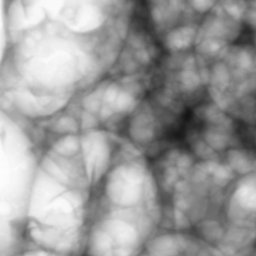
\includegraphics[scale=0.635]{figures/sim_foam.png}}
    \mbox{\vspace{15pt} 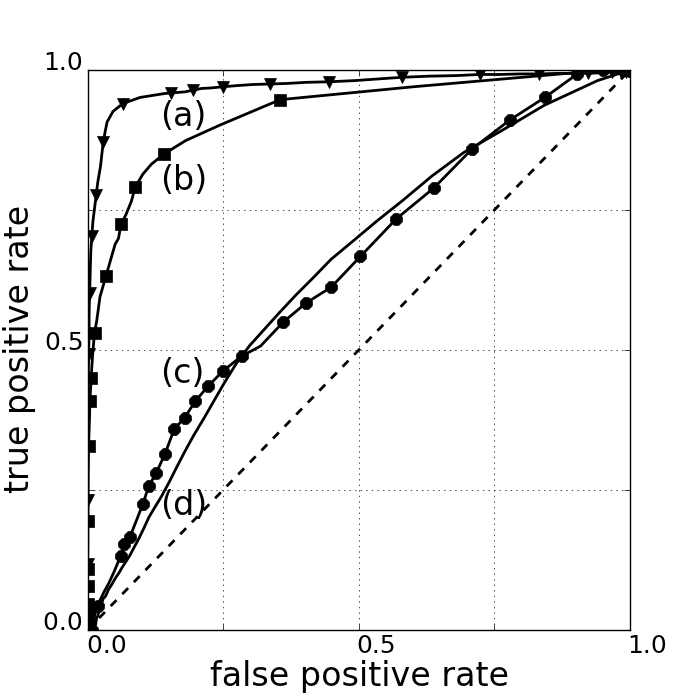
\includegraphics[scale=0.26]{figures/image_roc_all_methods_v3.png}}
  }
  \caption[]{Example of ROC curves analysis of coalescence detection methods. \textbf{Left:} Simulated radiograph. \textbf{Right:} ROC curves on simulated data for the simple difference approach \textbf{(d)}, the difference approach extended with morphological
operations \textbf{(c)}, the Fourier shift detection approach \textbf{(b)} and variational
optical flow with the forward-backward check \textbf{(a)}.}
  \label{fig:foam_performance}
\end{figure*} 

The quantitative evaluation of several coalescence detectors is given in Figure \ref{fig:foam_performance}. The curves represent the
receiver operation characteristic (ROC) of a given method,
which maps the false positive (fall-out) and true positive rates (sensitivity) for different thresholds parameters. The dashed line denotes the
ROC curve for the worst possible detector, which classifies the events equivalently to a random guess with the uniform distribution.

For the comparison we check the performance of four coalescence
detectors: (i) a simple difference approach, (ii) difference
extended by morphological filtering, (iii) Fourier shift detection
method \cite{Myagotin09}, and (iv) our proposed
variational optical flow approach combined with a forward–
backward check.

Inspecting the ROC characteristics it is evident that both difference-based approaches are unable to provide high detection quality. As a single measure of method accuracy we may use an area under the ROC curve (AUC). For difference-based methods it does not attain 0.7, while based on the theory of signal detection the value 0.75 assumed to be a acceptable classifier \cite{Swets88}. Motion-aware Fourier shift detection is
much more reliable even for the sequence with non-linear distortions (AUC = 0.93).
The proposed method, based on high
accuracy optical flow based, significantly outperforms other methods. Its estimated AUC value is in the range of 0.97-0.98 for all input sequences, which is close to ideal detector.  

In the next section we demonstrate a number of studies, in which
optical flow combined with the forward–backward
check is used as an analysis tool to perform
coalescence studies and to assess the stability of evolving
foams. In particular, we consider aqueous, metal and polymer
foam samples monitored by X-ray radiography.
 


\subsubsection{Results: Aqueous Foams}
\label{foam_aqueous}

The first application example of the devised optical flow detection technique is an automatic detection and registration of individual pore
collapses. For our X-ray experiment on aqueous foams we generated a long radiographic sequence consisting of 500 frames and depicting the
evolution of foam. Due to high stability of the
sample only a few collapses occur throughout the whole sequence. 
On Figure \ref{fig:foam_aqua} we present two typical cases of bubble rearrangements.


\begin{figure*}[ht]
  \centerline{
    \mbox{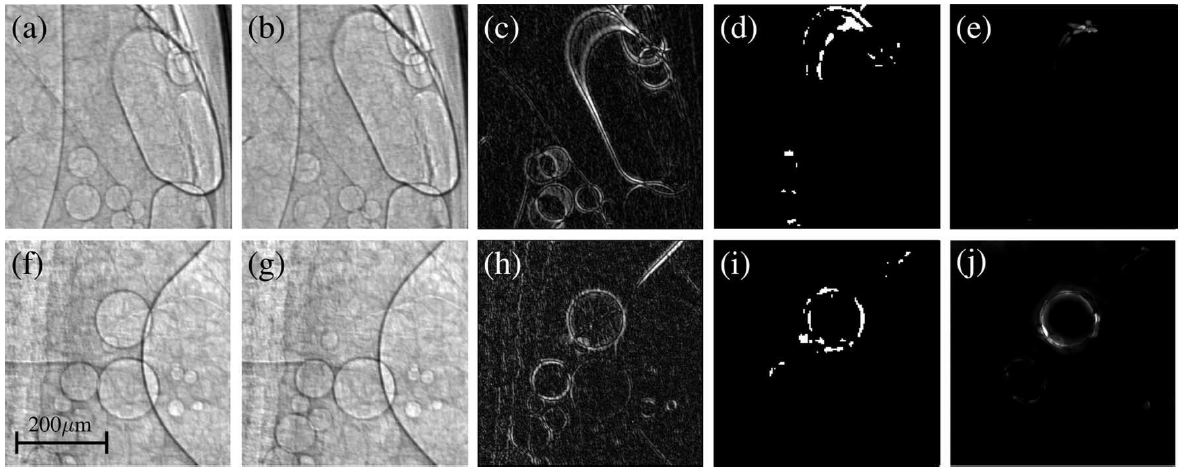
\includegraphics[scale=0.51]{figures/foam_aqua.png}}
  }
  \caption[]{Detection of single coalescence events in aqueous foam. \textbf{Top Row:} Displacement of foam constituents, no coalescence events. \textbf{Bottom Row:} Collapse of a bubble
combined with the motion of foam interior. \textbf{(a, b)} and \textbf{( f, g):} original successive radiographs; \textbf{(c, h):} difference
images between the two successive frames; \textbf{(d, i):} coalescence maps produced by the Fourier shift detection; \textbf{(e, j):} coalescence maps produced by the optical flow based. Both difference images (c, h) contain strong motion-related artifacts, which are also partly present in (d, i), while the map (j) correctly identifies the underlying bubble collapse and gives no false detections}
  \label{fig:foam_aqua}
\end{figure*}

The top row of Figure \ref{fig:foam_aqua}(a)–(e) corresponds to the case where only displacements
of foam constituents are present and no coalescence events happen. The images in the bottom row in Figure \ref{fig:foam_aqua}(f)–(j) show the collapse of a bubble
combined with the motion of surrounding constituents between the successive frames Figure \ref{fig:foam_aqua}(f, g). The difference method  in Figure \ref{fig:foam_aqua}(c, h) do not make the detection correctly since it produces a lot of false alarms because of structural motion and distortions. The detection method using Fourier analysis 
(Myagotin et al. 2009) performs better (Figure \ref{fig:foam_aqua}(d, i)),
but still includes a number of artifacts. The developed approach is able to distinguish pore collapses from simple rearrangements in
a much reliable manner (Figure \ref{fig:foam_aqua}(e, j)) This is also constituent with the results of performance evaluation using ROC curves analysis on synthetic dataset (see Section \ref{app_foams_performance}).


\subsubsection{Results: Metal Foams}
\label{foam_metal}

In this section we show \textit{in situ} coalescence analysis of metal 
foaming and capture spatial distribution of bubble collapses, which allows to assess evolution of foams for different mold geometries. In the following experiment two baking cups made from steel are used. We select two mold geometries for which completely different foaming behavior is presumed - wedge-shaped and L-shaped molds, each 10 mm in depth. On Figure \ref{fig:app_foams_maps} a time-lapse sequences of foaming process and estimated velocity vector fields are shown. 
\begin{figure*}[ht]
  \centerline{
    \mbox{\includegraphics[scale=0.95]{figures/app_foams_maps.png}}
  }
  \caption[]{Estimated velocity fields for two metal foaming geometries at different expansion stages. \textbf{Left column:} foaming in a wedge-shaped mold. \textbf{Right column:} foaming in an L-shaped mold. Plots \textbf{(e)} and \textbf{(j)} show integral coalescence distributions. The vertical coalescence event profiles reveal a lower events fraction in the bottom foam layers, where
film thinning is slowed down by a liquid material flow from upper layers.}
  \label{fig:app_foams_maps}
\end{figure*}
At the beginning samples expand mostly on the left-hand
side producing bumps of semi-liquid material. This is a result of
a non-uniform heating inside the molds. With the
course of time the right-hand foam front overtakes that on the
left-hand side. In the final expansion stage we observe a slow
continuous flow of the foamed material oriented parallel to
the inclined border in the wedge-shaped mold (Figure \ref{fig:app_foams_maps}(d)) and along
the cavity to the left and upwards in the L-shaped one (Figure \ref{fig:app_foams_maps}(i)). As expected, foams in wedge-shaped and L-shaped molds behaved differently.


Now we investigate spatial distribution of coalescence events. For this purpose we constructed integral coalescence maps for both samples.
The corresponding plots are demonstrated in Figure \ref{fig:app_foams_maps}(e) and
Figure \ref{fig:app_foams_maps}(j). Additionally, the horizontal and vertical integral coalescence
distribution histograms are plotted. A vertical event distribution
reflects a smaller number of collapses on the bottom and a higher fraction of events in the middle part of samples, as to be expected. The downward liquid flows (induced mostly by gravitational forces) supply the bottom layers of the foam with liquid melt. This delays the thinning of the bottom foam films, and produces the vertical gradient of coalescence events. The estimated data
are well in accordance with data estimated earlier (Babcsa´n et al., 2007).


The horizontal plots reveal an
anomalous and unpredictable effect. One recognizes
a high fraction of coalescence
events on the right-hand side of the
wedge-shaped sample (Figure \ref{fig:app_foams_maps}e)); in the plot (j) in Figure \ref{fig:app_foams_maps}
we observe an increased fraction of
coalescence events in the middle and on
the left- and right-hand sides of the
mold. The corresponding image regions
are highlighted by the grey rectangles in Figure \ref{fig:app_foams_maps}.
The possible interpretation of this effect
could be a low foam stability due to
 significant friction forces between
the upward moving foam front and the
steel mold. Friction forces promote film
stretching and additional topological
rearrangements of the foam films which
destabilize the foam structure, especially
at the mold’s faces. The important result of this
observation is that already
during the manufacturing stage of lightweight
components one can predict the
locations of possible detachments of the
metal foam from the requested profile.




\subsubsection{Results: Polymer Foams}
\label{foam_polymer}

A common receipt to improve the stability of foams is to include solid particles in the liquid phase. The particles are thought to increase the viscosity of the liquid and thus stabilize cell walls (Verdejo et al., 2009). In this section we analyze this technique by comparing
unfilled and filled silicone polymer foams. To provide quantitative information about foam stability we analyze temporal distribution of coalescence events.

For the experiment foaming takes place at room temperature as an exothermic reaction. Foaming takes place at room temperature as an exothermic reaction. Aligned multiwalled carbon nanotubes (MWNT) were synthesized in-house
by a chemical vapour deposition (CVD) technique. 
The carbon nanotubes were dispersed by high shear mixing in the polymethylhydrogensilane reactant. The two compounds were then mixed at a 1:1 ratio for 1 min. To study foam stability we consider two samples containing 0 and 0.2 wt\% of nanotubes (MWNT), called hereafter CONT and CVD, respectively.


In order to quantify coalescence processes, a running average for the coalescence rate (a)(t) and integral coalescence
fraction A(t) are plotted for both samples in Figure \ref{fig:foam_polymer}.

\begin{figure*}[ht]
  \centerline{
    \mbox{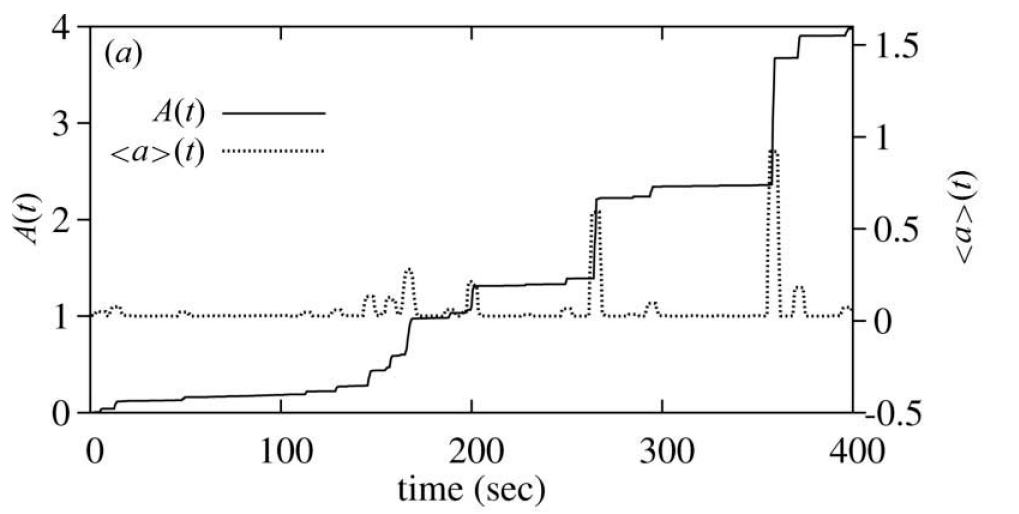
\includegraphics[scale=0.9]{figures/app_polymer_1.png}}
    \mbox{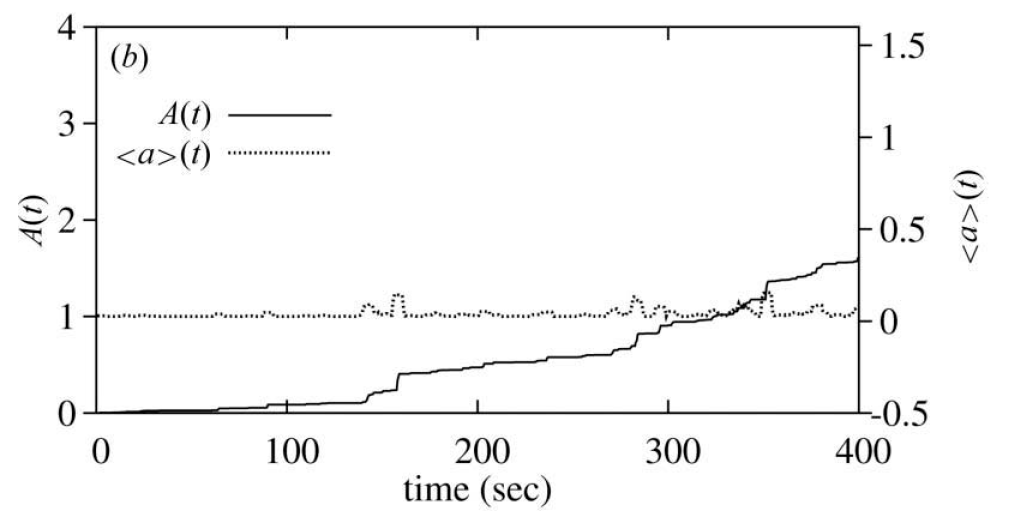
\includegraphics[scale=0.9]{figures/app_polymer_2.png}}
  }
  \caption[]{Coalescence rates for two kinds of polymer foams. \textbf{Left:} CONT sample (0 wt\% of MWNT  nanotubes). \textbf{Right:} CVD sample (0.2 wt\% of MWNT  nanotubes)  (all characteristics
are given in arbitrary units). A lower slope of the integral coalescence
fraction A(t) in the case of the CVD foam shows evidence of a higher
stability of the foam filled with nanoparticles.}
  \label{fig:foam_polymer}
\end{figure*}

The former  measure corresponds to the number of pixels covering
detected coalescence area. The latter is the total coalescence
rate (a)(t) integrated over a time period [0, t]. The
formal definitions and interpretations for these characteristics are given in
Myagotin et al. (2009). For both samples, already short after the onset of foaming the first coalescence events are detected which are
represented by peaks on the coalescence rate (a)(t) plot. With the course of time the two samples evolve differently. Exploring the plots, it becomes evident that in the case of CONT foam sample relatively rare events happen with rather high amplitude (large detected area) which indicates large coalescing bubbles.


The integral coalescence of the CVD sample, in contrast, is
a more linearly increasing function, which shows an almost constant
number of low-intensity film ruptures per unit time. Comparing the two samples one may notice that the CONT foam exhibits a significantly higher integral coalescence than CVD sample.
These observations support the hypothesis that, owing to an
increased viscosity of the liquid or decoration of the cell walls
by the nanoparticles, capillary drainage in the filled sample is
significantly reduced. This in turn leads to a reduced film
thinning rate and to more stable liquid films separating the
bubbles, and consequently to more stable foams.

By the systematic use of X-ray radiography combined with optical flow it is possible to analyze coalescence processes for
a diversity of foam types. By introducing a concept of the
forward–backward check we are able to increase reliability of detection
reliability and improve quantification of coalescence events.
The presented approach is suitable for the detection and
localization of individual film or bubble collapses, as well as for
the estimation of spatial and temporal distributions of the
coalescence events. These studies can provide insights about the underlying processes of foaming dynamics which is important for understanding of physics of foams and their production.







         
%\subsection{[OPTIONAL] Inspection of flip chip devices}


%\section{Registration of joints movement in insect}
%            Image registration

\newpage


\section{Tracking}

\subsection{Kinematics Analysis of Joint Parts in Living Insect}
\label{app_kinematics_insects}


\subsubsection{Introduction}

\textit{Arthropods} are the most numerous species and constitute more then 80\% of all animals. Biologists have a major interest in studying their morphological diversity and related physiology. However, remarkably little is known about their functional morphology. The main reason is, until recently there has been no imaging method, which allows \textit{in vivo} investigation of internal structures in 3D and real-time for non-transparent organisms such as most arthropods.  

For optically opaque living organisms X-ray imaging methods are ideal techniques due to the high penetration ability of the radiation. For \textit{static} specimens synchrotron-based X-ray computed microtomography (SR-$\mu$CT) has proven to be a powerful tool to study arthropod morphology \cite{Westneat08}. To analyze \textit{in vivo} dynamics of internal structures sequences of 2D X-ray projection radiographs were recorded \todo{Change}[Ref 7,8]. However, in this case the depth information is lost, structures are superimposed, which complicates their identification and analysis.  

Recently, a system for in vivo X-ray cine-tomography was designed, which aims to  investigate previously inaccessible 3D morphological dynamics with feature sizes in the micron range and with temporal resolution down to a fraction of a millisecond \cite{dosSantosRolo14}.  An important component of the X-ray 4D cine-tomography is not only an image acquisition system, realized by means of ultra-fast SR-$\mu$CT, but also an automated data processing and motion analysis procedures. This combination allows to provides complete 4D quantitative information on the functional morphology of the living specimen.


\subsubsection{Experimental Setup}

Data acquisition was performed at the TOPO-TOMO
beamline at the ANKA synchrotron facility operated by Karlsruhe Institute of Technology. A white X-ray beam was filtered by 0.2 mm aluminum plate giving a photon energy window of 9.6 - 24 keV with the maximum flux density at 14.5 keV.

The indirect X-ray detector system was optimized to achieve an effective pixel size of was 1.2 $\mu$m, with a field of view of 2.464 mm. A camera system is a pco.dimax CMOS camera with 2016$\times$2016 pixel resolution.



\begin{figure*}[ht]
  \centerline{
    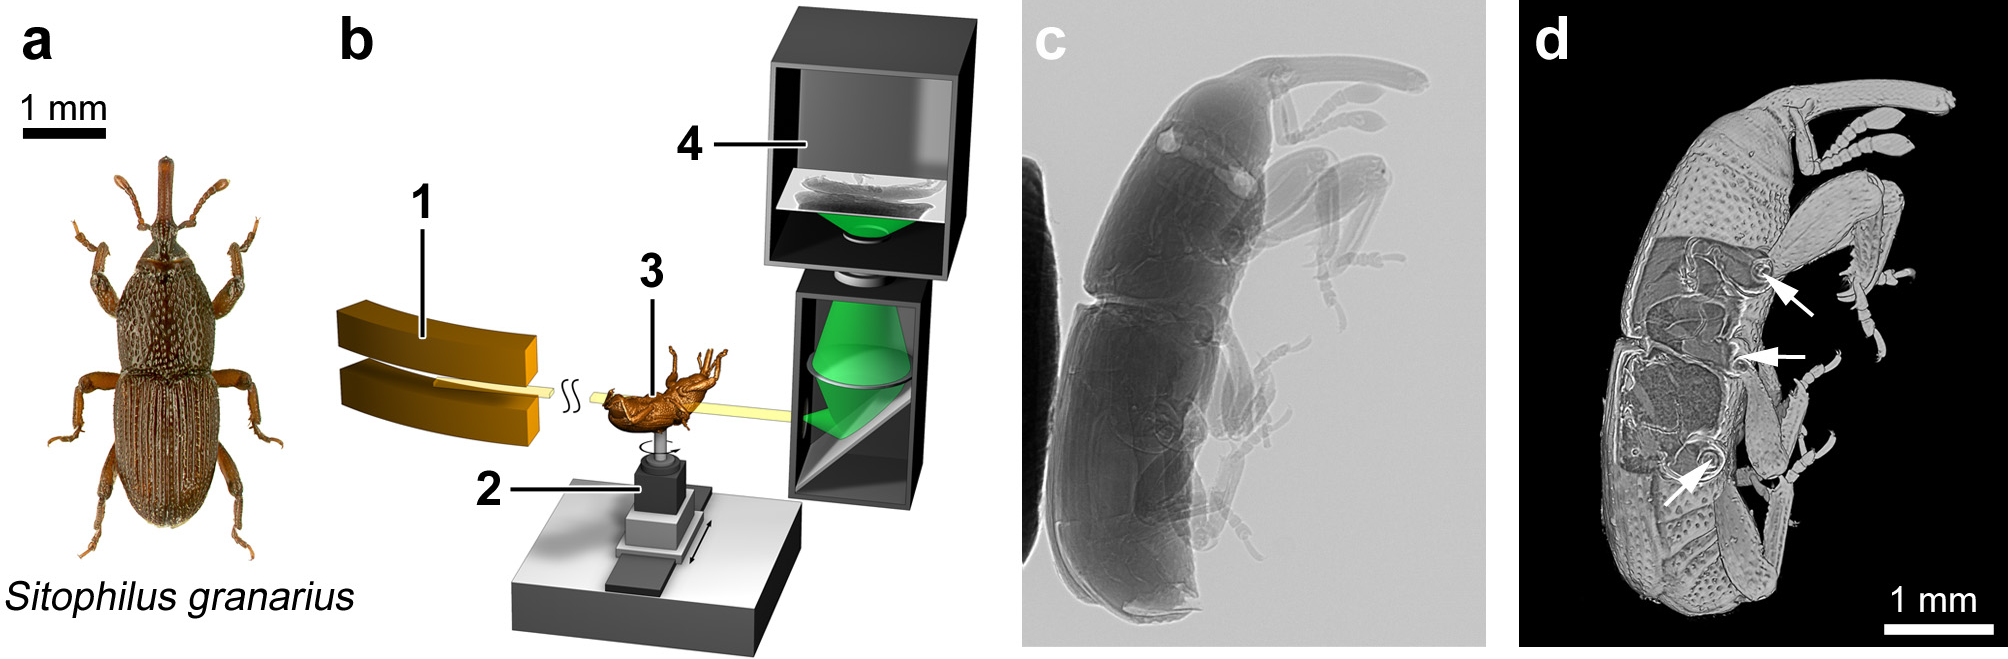
\includegraphics[scale = 0.225]{figures/app_bug_setup.PNG} 
  }  
  \caption{In vivo X-ray 4D cine-tomography experiment. \textbf{(a)} Photograph of Sitophilus granarius, dorsal
view. \textbf{(b)} Experimental set-up for ultra-fast X-ray microtomography showing bending magnet (1),
rotation stage (2), fixed specimen (3) and detector system (4). \textbf{(c)} Radiographic projection. \textbf{(d)} 3D
rendering of the reconstructed volume with thorax cut open and revealing hip joints (arrows).}
  \label{fig:app_bug_setup}
\end{figure*}

Static overview radiographs (Figure \ref{fig:app_bug_setup}c) and reconstructed tomographic images (Figure \ref{fig:app_bug_setup}d) were acquired using a detector system
equipped with a Photron SA1.1 camera. The resulting pixel size was 6.6 $\mu$m,
with a field of view of 6.6 mm. These images were used to examine the insect's internal structures and identify location of the region of interest (screw-and-nut joint system, see arrows in Figure \ref{fig:app_bug_setup}d).




To acquire \textit{in vivo} tomograms of moving weevil and roughly estimate parameters of its motion, the specimen was imaged with a temporal resolution of 20 tomograms per second by 
continuous rotation with 10 revolutions per second. The camera recording frame rate was 5.000 frames per second and 250 projections were used per tomogram. The distance between sample to detector was 50 cm.

As the last level of our data acquisition pipeline we recorded high resolution radiographs of moving hip joint region (Figure \ref{fig:app_bug_motion_seg}a-c) while the specimen was continuously rotating with 3.25 revolutions per second.
The images were recorded with a rate of 1500 frames per second. To acquire one tomogram we used 200 radiographs, instead of 250 for high-speed tomographic setup, the resulting temporal resolution was 7.5 tomograms per second. The sample to detector distance was 20 cm.
A combination of these parameters was a good compromise between fast acquisition time and image resolution, which allowed us to study both structure and dynamics of the screw joint. 

Additionally, after \textit{in vivo} data acquisition, the same specimen was scanned \textit{post mortem} (Figure \ref{fig:app_bug_motion_seg}d) to obtain high-quality static
volumes of the joint region. For this case we increased the exposure time and 1000 projections were collected with a frame rate of 100 frames per second.


\subsubsection{Task for Data Processing}

The main task for data processing is a quantitative kinematics analysis of two parts of a hip joint: coxa (hip)
and trochanter. 

For this purpose we perform:
\begin{itemize}
	\item Motion estimation to track individual parts of the hip joint.
	
	\item Visualize morphological structures in 3D.
	
	\item Extract kinematics parameters: global coxa movement, rotation of the trochanter and translation of the trochanter inside the coxa.
	
\end{itemize}


\subsubsection{Data Evaluation}

Before we proceed with a development of a data processing workflow, which is required to accomplish the task of quantitative estimation of kinematics in the joint system of a living bug, we evaluate the screw joint dataset according to our data taxonomy: \ref{data_taxonomy}:

\begin{itemize}
	\item \textit{Image noise}: The original radiograms contain high amount of noise due the short exposure time, which was necessary to limit radiation damage to the sample. After the tomographic reconstruction the amount of noise is reduced. However, the image data still suffers from the presence of noise. Therefore a dedicated preprocessing routine to perform noise reduction is required. Moreover, an optical flow model which is robust with respect to noise should be used. 
	
	\item \textit{Contrast level}:  The image contrast is low, different structures of the joint system are hardly resolved between each other (See Figure \ref{fig:app_bug_motion_seg}). A proper treatment of low-contrast data is needed. The employed optical flow model should be adjusted to low-contrast data. The insufficient contrast is the major challenge of this dataset.
	
	\item \textit{Object size}: The structures the joint system are of different sizes. In general, according to our data classification, they can be describe as average. 
	
	\item \textit{Object distribution}: Different parts of the joint system are distributed normally.
	
	\item \textit{Object details}: The amount of feature in various parts of inner structures is not sufficient. All parts are depicted as homogeneous structures (See Figure \ref{fig:app_bug_motion_seg}). Low amount of image details is the second main challenge of this dataset.
	
	\item \textit{Image artifacts}: The main source of image artifacts is motion blur. Since during this in vivo experiment, the bug was moving, the acquisition parameters were adjusted in such a way that to achieve a compromise between dose, temporal resolution, image contrast and signal-to-noise ratio. As a result, temporal resolution was not sufficient to allow to follow fast movements in real time. After the image reconstruction motion-related artifacts emerge.  In order to compute reliable optical flow the artifacts should treated. Otherwise, the artifacts could obstruct the successful application of optical flow methods.  
	
	\item \textit{Motion type}: The motion of the screw joint and other structures is strictly rigid. The trochanter (an actual screw) undergoes fast rotation, as well as the translation within the coxa part (a box that contains the screw). Using the rigidity assumption we can design a special tracking procedure, which allows to overcome problem with image artifacts or insufficient amount of image details (see next sections).
	
	\item \textit{Motion range}: Rotation of the trochanter structure is very fast, depending on a distance to the axis of rotation. However, the translational part of the movement is relatively slow. These aspects should be taken into account when modeling a motion estimation procedure.
	
	\item \textit{Motion discontinuities}: The amount of motion discontinuities is normal and should not cause any problems for the optical flow estimation.
\end{itemize}




A summary of evaluation of screw joint dataset is given in Table \ref{tab:eval_screw}.
\begin{table}[ht] \footnotesize
	\centering
	\caption{Evaluation of the screw joint dataset.}
	\begin{tabular}{ccc}
		\toprule
		\textbf{Image} & \textbf{Data}   & \textbf{Motion}   \\ 
		\midrule
		\cellcolor{bad} noise: high         & \cellcolor{norm} size:  average  & \cellcolor{good} type: rigid    \\ 
		\cellcolor{bad} contrast: low         & \cellcolor{norm} dist: norm            & \cellcolor{bad} range: mixed  \\ 
		\cellcolor{bad} artifacts: motion   & \cellcolor{bad} detail: low  &  \cellcolor{good} disc: norm   \\ 
		\bottomrule
	\end{tabular}
	\label{tab:eval_screw}%
\end{table}


\textbf{Requirements on the Results}
\\
\\
\textit{Accuracy}: For this dataset we require accurate results. Since the main task is to reconstruct the kinematics of the screw joint system over period of time, we require accuracy not only between two successive frames, but also for the whole motion cycle.  The error in the range of 1-2 pixels would be sufficient for a pair of images, but exceeding values should be eliminated from the results or indicated. For the whole sequence the error of more then 5-7 pixels is already a substantial mistake, if the structure have displaced for around 20 pixels. In other world the total error depends on the total displacement and should not exceed 25\%.
\\
\\
\textit{Density}: Dense flow fields are not required, since the main task is to reconstruct motion components (rotation and translation) during the movement. The fact that this requirement is relaxed gives the possibility to evaluate the computed flow field, filter unreliable flow vectors using internal confidence measures and perform analyses of flow components using a sparse flow field. 
\\
\\
\textit{Motion components}: The full flow is required, i.e. both the flow magnitude and the flow direction. 
\\
\\
\textit{Consistency}:  The assumption, that the flow vectors are consistent in the forward and backward directions is the main idea behind our approach to filter unreliable flow vectors (see the description of data processing workflow).
\\
\\
\textit{Motion boundaries}: We do not aim to capture strict flow on the boundaries of moving structures. Only general information about each structure is required - location, translation and rotation from the previous frame.
\\
\\
\textit{Computation time}: Computation time is not an issue, the processing is done offline. Taking into account the size of tomographic datasets, it is advantageous to perform the computation on GPU.
\\
\\
\textit{Data size}: The original size of a single tomogram is 2016 $\times$ 2016 $\times$ 2016, \todo{Check numbers} which corresponds to 32 Gb of floating-point data. Each pair of the image sequence can be stored in the memory both on CPU and GPU. 



\subsubsection{Data Analysis: Preprocessing}

\noindent \textit{Flat-filed correction}. Before tomographic reconstruction, the original radiographs were normalized by flat field correction \ref{flat_field_correction}. 
\\
\\
\textit{Noise filtering}. Due to the short exposure time during fast acquisition
process the images are contaminated with high amount of noise. Prior to tomographic reconstruction we perform a noise filtering. 
Another challenge with respect to image quality is a low separation contrast between different structures. This should be taken into account for the design of filtering procedure. As an example, image denoising using the Gaussian low-pass filtering is a common approach (see Section  \ref{noise_filters}). However, the filter restores the pixel value by averaging its
spatial neighborhood, thus blurring important image details. For this reason an edge-preserving filtering approach is desirable.

In the review of image denoising algorithms a non-local means algorithms (NLM) was presented \cite{Buades05}. It was shown that NLM algorithm gives minimum mean-square error between the noisy and the uncorrupted image for signal-independent additive white
noise. Additionally, in the comparison with other methods such as Gaussian filter, anisotropic filter and total variations (TV), NLM algorithm showed better performance.  

However, as we discussed in Section \ref{noise_filters} for X-ray data the most influential noise model is described by a Poisson distribution, and
Poisson noise is not independent of the signal intensity, as required for NLM methods.
For this reason we perform a noise variance
equalizing transformation \todo{cite} before noise filtering \todo{Ask Tomy what is that}. After the noise removal by NLM algorithm, feature details are preserved and high-frequency noise is significantly decreased.
\\
\\
\textit{Tomographic reconstruction}. 3D image reconstruction is performed using the filtered back-projection method (see Section \ref{computed_tomography}) using a Ramp filter \cite{Buzug08}. This approach differs from a conventional filtering during back projection procedure, when Shepp-Logan or the Hamming filters are used \cite{Buzug08}. Both filters allow to reduce noise by dumping high spatial
frequencies. However, in our preprocessing procedure we use a separate noise filtering step, which allows us to employ a non-windowed
filter function. As a consequence, image feature are better preserved, as required for motion estimation.
The reconstructed 3D images can still be degraded by motion artifacts, since no motion-aware reconstruction was used. To tackle with the remaining artifacts a robust optical flow computation method is employed.



\subsubsection{Data Analysis: Motion Computation}

To capture dynamics of the screw-and-nut system we develop a robust 3D variational optical flow method. It is designed to be
robust against image artifacts and yet be sensitive to low-contrast image
details represented different structures. For the data term we use constancy of image brightness \ref{brightness_constancy_assumption}. Instead of
using a common total variation (TV) approach to model the data term (robust approach \ref{robust}), we employ
quadratic penalization to enhance the contribution of image gradients
(representing boundaries between structures), which were deliberately and carefully preserved throughout the entire image processing and reconstruction pipeline (see noise filtering and reconstruction steps).
Since motion artifacts could still appear within image data, to discard them we selectively model data constancy using an automated confidence measure based on cross-checking \ref{forward_backward_check}.  A first computation of optical flow  is performed to localize data outliers and construct a confidence map for each pixel position.  This confidence map is then applied during the second run of optical flow algorithm to reduce the contributions from problematic image areas and thus to refine the
motion field \ref{refinement}.
We further improve robustness of data term against noise using
a combined local–global approach \ref{clg}, which takes in account an information from a local region. Large value of integration scale is used, with the optimal value in the range $\rho = [0.7 \ldots 1.5]$. 
For the regularization of the motion field we use a combined image
and flow-driven smoothness method \ref{image_flow_smoothness}. This approach imposes more
strict smoothness constraints inside homogeneous image regions, but preserves
motion boundaries near separate structures. Again, large values of smoothness parameters are required to give reliable results.  

To capture the entire range of movements, including fast rotation of the
trochanter, we use a multi-level computation procedure. The parameters are the same as for \textit{baseline} model \ref{baseline_method}.  Between computation levels we use median filtering \ref{flow_median} with large spatial mask ($m=5$) to suppress data outliers from coarser levels.

\begin{figure*}[ht]
  \centerline{
    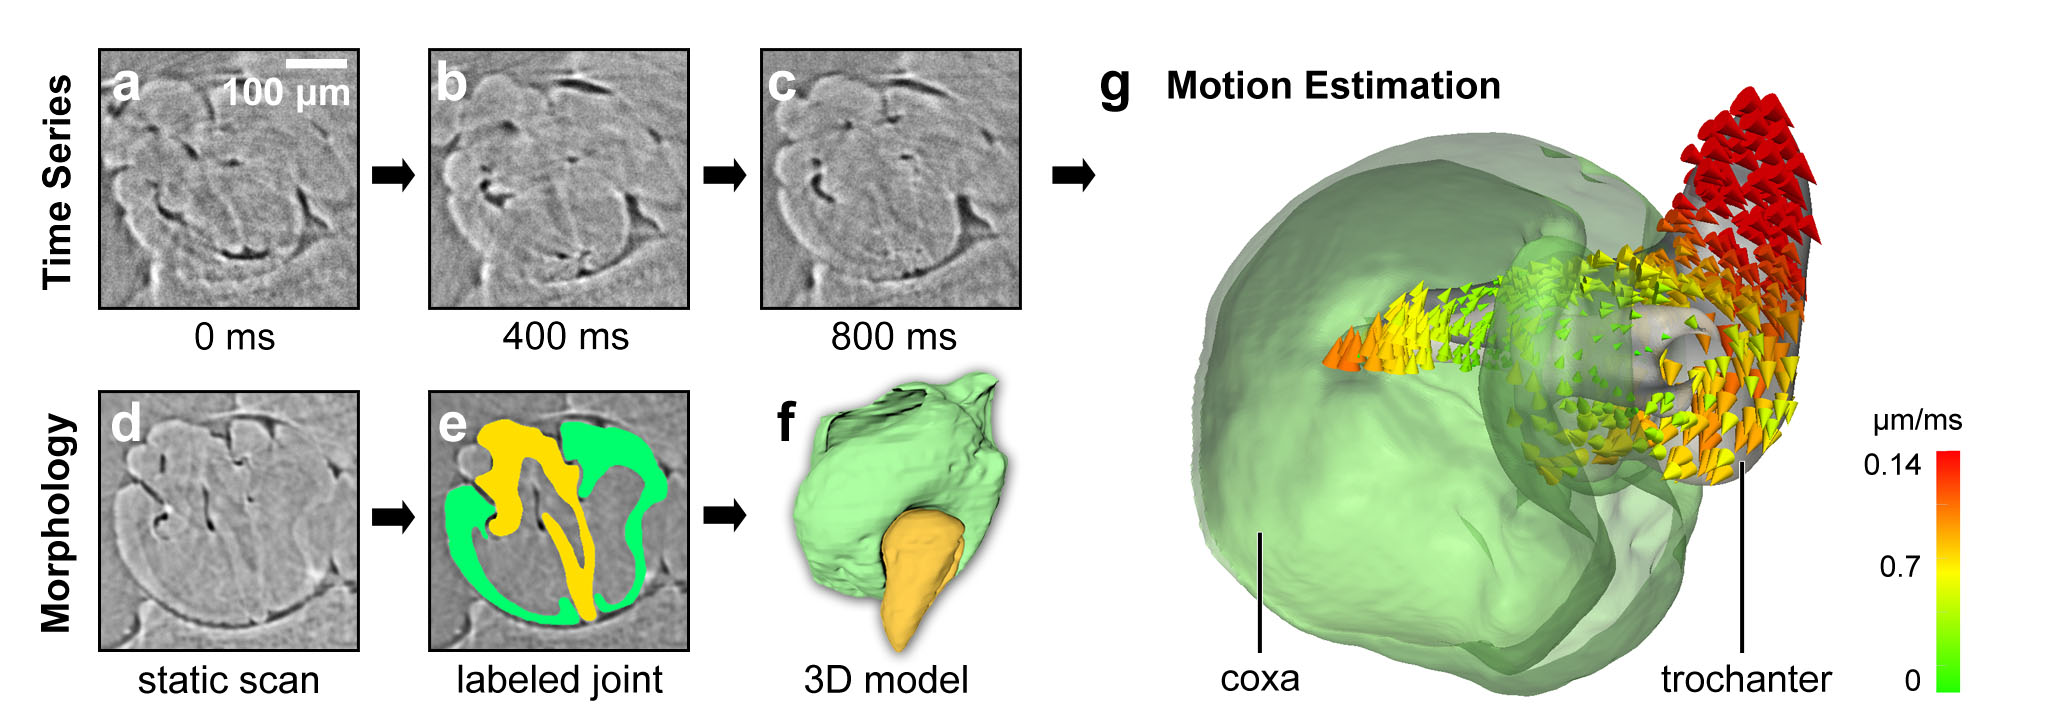
\includegraphics[scale = 0.228]{figures/app_bug_motion_seg.PNG} 
  }  
  \caption{Morphological dynamics and kinematics analysis of the screw joint during defensive movement. \textbf{(a-c)} Time-lapse
sequence of tomographic slices for times 0, 400 and 800 ms, respectively. \textbf{(d)} Tomographic slice of \textit{post
mortem} scan with increased exposure time and, as a result, image contrast. \textbf{(e)} Manual labeling of coxa (green) and trochanter
(yellow). \textbf{(f)} 3D model of the screw joint based on manual labeling. \textbf{(g)} 3D motion field computed
from 0 ms and 130 ms and represented as 3D glyphs colored according to magnitude}
  \label{fig:app_bug_motion_seg}
\end{figure*}

\subsubsection{Data Analysis: Tracking}

To perform a fully automated tracking of individual parts of the screw joint we use the results of optical flow computation on subsequent volume images.
For the first frame of in vivo image sequence we automatically distribute 70 and 130 landmarks for coxa and trochanter, respectively. Part of the landmarks (50 \%) were placed using a grid with equal spacing to uniformly cover both joint parts. The locations for rest of landmarks were selected based on image edges \ref{tracking}. For each landmark $L_t(\textbf{x})$ at a
time frame $t$, the corresponding landmark on time frame $t+1$ is provided by the displacement vector $\textbf{u}(\textbf{x})$. 

In order to improve accuracy of the tracking procedure we filter unreliable trajectories using a forward-backward
cross-check \ref{forward_backward_check}. This method ensures consistency of tracking results computed in forward and reversed directions by evaluating the difference between the location of initial landmark and its position followed in
opposite direction a possible errors could be identified (see Figure \ref{fig:app_bug_cross_checking}). We eliminate data points with the discrepancy of forward-backward check of more then 3 pixels tracked throughout the entire sequence. 
As an additional constraint we perform rigidity
check by analyzing relative spatial arrangement of landmarks \ref{object_tracking}. We filter out  30\% of landmarks showing the most
deviations from rigidity constraint. The remaining high-confidence landmarks  are used to estimate global transformations of moving joint parts.


\begin{figure*}[ht]
  \centerline{
    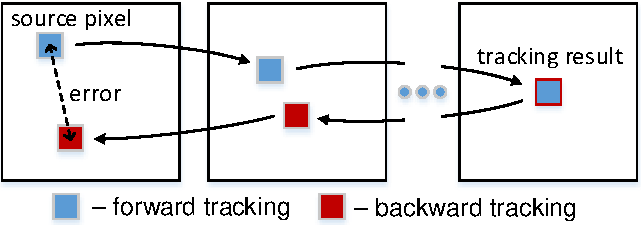
\includegraphics[width=0.6\textwidth]{figures/fig_620_p185.pdf} 
  }  
  \caption{Cross-checking principle.}
  \label{fig:app_bug_cross_checking}
\end{figure*}


\subsubsection{Data Analysis: Kinematics}
\label{bug_kinematics}

For the estimation of global transformation between two sets of landmarks and
extraction of motion components we use a dedicated Python module for matrix transformations \url{http://www.lfd.uci.edu/~gohlke/}.  A transformation matrix $M_t$, which performs rigid transform of landmark positions between successive time frames, was calculated using Kabsch algorithm \cite{Kabsch76} (See Section \ref{transform_estimation}). The resulting
matrix was then decomposed to extract translational and rotational components (Figure \ref{fig:app_bug_kinematics}i). 

For the trochanter part, displacement towards the coxa and rotation angles are evaluated with respect to its longer axis on the first time frame.
To check the accuracy of automated tracking via motion analysis we compared it with a manual tracking performed by the expert.  We achieved an average error for coxa displacement of 0.7 pixels with the average
/ maximum actual displacement of 3.7 / 5.2 pixels; an average error for trochanter displacement of
3.7 pixels with the average / maximum actual displacement of 10.7 / 18.0 pixels; an average error of
trochanter rotation of 2.5 degrees with the average / maximum actual rotation of 55.4 / 94.8 degrees. Such performance in terms of accuracy was sufficient for a fully automated tracking procedure.


\begin{figure*}[ht]
  \centerline{
    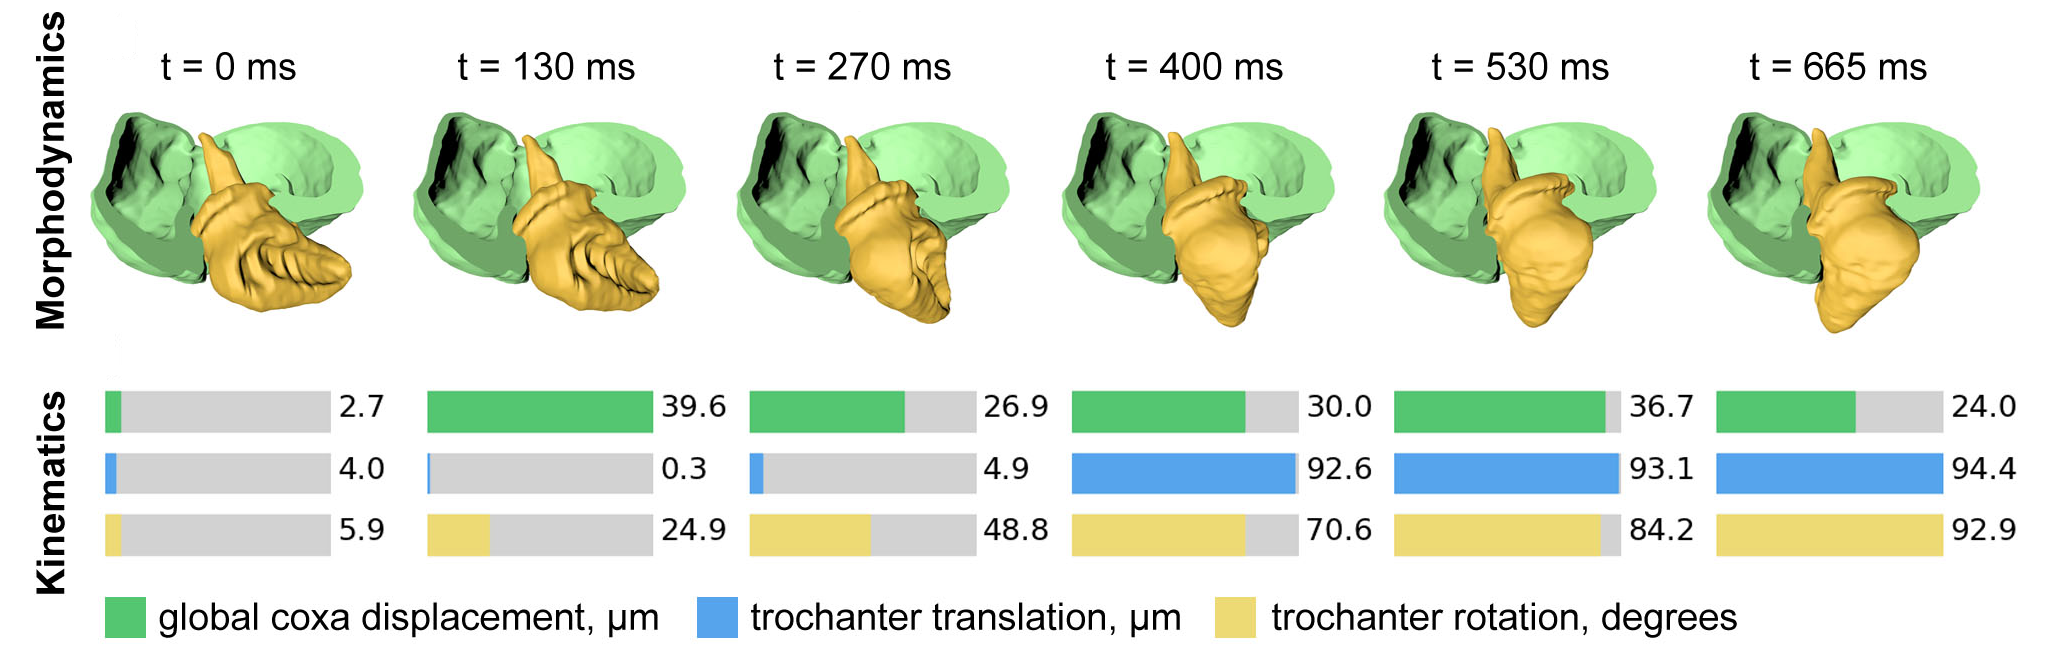
\includegraphics[scale = 0.228]{figures/app_bug_kinematics.PNG} 
  }  
  \caption{Morphological dynamics and kinematics analysis of the moving screw joint. \textbf{Top row}: \textit{In vivo} dynamics of joint parts based on the 3D segmented static model \ref{fig:app_bug_motion_seg}f and automated tracking with motion analysis \ref{fig:app_bug_motion_seg}g. \textbf{Bottom row}: Analysis of kinematics. Global
displacement of the whole screw-and-nut system with respect to the main body (green plot); fast translation of the trochanter inside the coxa (blue plot);
linear rotation (screwing process) of the trochanter (yellow plot).}
  \label{fig:app_bug_kinematics}
\end{figure*}

To visualize morphological parts in dynamics the 3D volumes of the static and the first frame of in-vivo scans were imported into the data analysis software Amira 5.4. Coxa and trochanter parts were then labeled manually. Next, coxa and trochanter from the static scan were aligned manually to match the first frame of the in vivo scan. The high quality labeled data from the static scan was then transformed according to its actual
motion calculated during kinematics analysis from the previous step \ref{bug_kinematics}. 
As a result we obtain an \textit{in vivo} quantitative morphological dynamics of moving joint parts.




\subsubsection{Results}


In this work we capture 4D spatio-temporal information about complex kinematics in living insect using optical flow and automated tracking, which allows us to visualize the functionality of internal structures (Figure \ref{fig:app_bug_kinematics}). To determine quantitative characteristics of screwing process we separate the angular velocities from translational motion of trochanter inside the coxa. 
The results show that the trochanter rotated within 0.8 s around 92.9 degrees clockwise (from the view point of
an outside observer) \ref{fig:app_bug_kinematics}. The rotation was accompanied with an inward translation along the axis of
rotation of 94.4 $\mu$m (Figure \ref{fig:app_bug_kinematics}). The relation between rotary and translatory movements appears to be nonlinear,
which can be a consequence of comparatively wide opening space observed between the trochanteral
and coxal thread. Such type of motion is unlikely for the narrow hip
joints described for \textit{Trigonopterus oblongus} \cite{vandeKamp11}, as the defensive strategy of the genus relies on
more narrow type of screw joints. Therefore, the current studies also provide an evidence for the functional
variability of the constriction of leg joints in weevils, which can be closely related to their ecology.

A X-ray 4D cine-tomography has been proven to be a promising tool to
study morphological dynamics in millimeter-sized animals such as insects and can be employed to investigator other biological
specimens and processes.


%\section{[OPTIONAL] Image Registration}
%\comment{Skip the whole section? Or maybe mention very briefly}
%\subsection{[OPTIONAL] Inspection of flip chip devices}


%\section{Registration of joints movement in insect}
%            Image registration

%\subsection{Water transport analysis in living bamboo plants}
%
%\comment{Could be skipped?}



